% +------- CÓDIGO FONTE TCC -------+
% 	Autor: Antônio Barbosa Neto, 2017.
% 	E-mail: abneto14@gmail.com
% +--------------------------------+

% Classe do documento --> \documentclass[OPÇÕES]{CLASSE}
\documentclass[
			   a4paper, % Tipo de papel 
			   oneside, % Impressão em apenas um lado da folha
			   12pt     % Tamanho da fonte
			   ]{book}  % Classe do documento

\usepackage{dashbox}
% Pacotes --> \usepackage[OPÇÕES]{PACOTE}
\usepackage[utf8]{inputenc} % Codificação do documento (conversão automática dos acentos) 
\usepackage[brazil]{babel}  % Traduz palavras chaves para o PT-BR (ex.: abstract->resumo)
\usepackage{indentfirst}    % Indenta o primeiro parágrafo de cada seção
\usepackage{setspace}		% Possibilita a alteração do espaçamento entre linhas
\usepackage{graphicx}       % Possibilita a inserção de figuras
\usepackage{subcaption}  % Possibilita a inserção de subfiguras
\usepackage{pdfpages}       % Possibilita a inserção de páginas em pdf
\usepackage{amsmath}        % Inclui funções adicionais no ambiente matemático \eqref{•} \dfrac{•}{•}
\usepackage{amssymb} 		% Símbolos adicionais no documento \mathbb{R}
\usepackage{amsfonts}
\usepackage{amsthm}
\usepackage{mathrsfs}       % Símbolos da transformadas de Laplace e Fourier \mathscr{•}
\usepackage{float}			% Possibila posicionar tabelas e figuras em uma posição específica [H]
\usepackage[round]{natbib}% Inclui mais possibilidades de citações \citep{•}
\usepackage{fancyhdr}       % Possibilita a alteração de cabeçalho e rodapé
\usepackage{longtable}      % Possiblita a quebra de tabelas em duas páginas
\usepackage{multirow}		% Possibilita multiplas linhas em tabelas
\usepackage{array}			% Possibilita o uso do comando \newcolumntype{•}[•]
\usepackage{pdflscape}      % Possibilita a inserção de páginas em modo paisagem
\usepackage{listings}		% Possibilita inserir códigos fontes (C++, Java, ...)
\usepackage{slashbox}       % Adiciona o comando \backslashbox{•}{•} usado em tabelas
\usepackage{arydshln}       % Possibilita inserir linhas pontilhadas em tabelas 
\usepackage{adjustbox}      % Possibilita ajustar as tabelas as margens
\usepackage{rotating}       % Rotaciona tabelas
% \usepackage[alf]{abntex2cite}	% Citações padrão ABNT

\usepackage{tikz}
\usepackage{courier}
\usepackage{booktabs}     
\usepackage{svg}

\newcommand{\PR}[1]{\ensuremath{\left[#1\right]}}
\newcommand{\PC}[1]{\ensuremath{\left(#1\right)}}
\newcommand{\chav}[1]{\ensuremath{\left\{#1\right\}}}

\newcommand{\commentiury}[1]{{\color{blue}[IB: #1]}}

%\usepackage[inline]{showlabels} % Mostra os labels das equações
%\usepackage[notcite,notref]{showkeys} % Mostra todo os labels
\usepackage{lipsum} % preenchimento automático de textos

% Modifica os itens do sumário
\usepackage[nottoc,
			notlof,
			notlot]{tocbibind}

% Configura as margens das páginas
\usepackage[top    = 3cm,
			bottom = 2cm,
			left   = 3cm,
			right  = 2cm]{geometry}

% Possibilita hiperlinks no texto
\usepackage[pdftex,
			% backref,
			linktocpage = false,
			colorlinks  = true,
			linkcolor   = black,
			anchorcolor = blue,
			citecolor   = blue,
			urlcolor    = blue]{hyperref}

      
\usepackage[acronym, shortcuts]{glossaries}
\makenoidxglossaries

% Comandos auxiliares --> \nomecomando{COMANDO}{•}
\newcolumntype{C}[1]{>{\centering\let\newline\\\arraybackslash\hspace{0pt}}m{#1}} % Tabelas: {|C{2cm}|C{5cm}|}
\newcolumntype{L}[1]{>{\let\newline\\\arraybackslash\hspace{0pt}}m{#1}} % Tabelas: {|L{2cm}|L{5cm}|}
\newcommand*{\doi}[1]{DOI: \href{http://dx.doi.org/#1}{#1}} % Usado nas referencias

\setcounter{secnumdepth}{3} % Inclui a numeração de \subsubsection{•} no documento
\setcounter{tocdepth}{3}    % Inclui a \subsubsection{•} no sumário
\setstretch{1.5}			% Configura o espaçamento entre linhas \usepackage{setspace}

\pagestyle{fancy} 			% Configura a página para incluir o cabeçalho e rodapé
\lhead{{\footnotesize\leftmark}} % Cabeçalho esquerdo
\chead{}				         % Cabeçalho central
\rhead{\thepage}				 % Cabeçalho direito
\fancyfoot{}					 % Rodapé vazio

% Definição de novas cores
\definecolor{mygreen}{RGB}{0, 115, 0}
\definecolor{mylilas}{RGB}{170,55,240}
\definecolor{blue}{RGB}{41,5,195}

% \lstset{ % -> \usepackage{listings}
%   language=Matlab,
%   basicstyle=\ttfamily\small, 
%   morekeywords={matlab2tikz},
%   keywordstyle=\color{blue}, 
%   stringstyle=\color{mylilas}, 
%   commentstyle=\color{mygreen}, 
%   extendedchars=true,
%   showspaces=false,
%   showstringspaces=false,
%   numbers=left,
%   numberstyle=\tiny,
%   breaklines=true,
%   breakautoindent=true,
%   captionpos=b,
%   xrightmargin=0pt,
%   xleftmargin=15pt,
% }

\renewcommand{\lstlistingname}{Código}
\lstset{
  language=Python,
  tabsize=2,
  basicstyle=\small\linespread{1.2}\ttfamily,
  keywordstyle=\bfseries\color[gray]{0.2},
  commentstyle=\color{darkgray}\textit,
  breaklines=true,
  breakatwhitespace=false,
  extendedchars=true,
  showspaces=false,
  showstringspaces=false,
  numbers=left,
  numberstyle=\tiny,
  breaklines=true,
  breakautoindent=true,
  captionpos=b,
  xrightmargin=0pt,
  xleftmargin=15pt,
  % inputencoding=utf8,
  literate={á}{{\'a}}1 {à}{{\`a}}1 {â}{{\^a}}1 {ã}{{\~a}}1 {é}{{\'e}}1 {ê}{{\^e}}1 {ë}{{\"e}}1 {í}{{\'i}}1 {ç}{{\c{c}}}1 {Ç}{{\c{C}}}1 {õ}{{\~o}}1 {ó}{{\'o}}1 {ô}{{\^o}}1 {ú}{{\'u}}1 {δ}{{\ensuremath{\delta}}}1 {Ξ}{{\ensuremath{\Xi}}}1 {Ψ}{{\ensuremath{\Psi}}}1 {Γ}{{\ensuremath{\Gamma}}}1 {λ}{{\ensuremath{\lambda}}}1 {θ}{{\ensuremath{\theta}}}1
}

% Novos comandos --> \newcommand{COMANDO}{DEFINIÇÃO}
\newcommand{\instituicao} {
  UNIVERSIDADE FEDERAL DO AMAZONAS \\
  FACULDADE DE TECNOLOGIA \\
  ENGENHARIA DA COMPUTAÇÃO 
}
\newcommand{\titulo} {
  CONTROLE BASEADO EM EVENTOS DE CONVERSORES CC-CC CONECTADOS A CARGAS DE POTÊNCIA CONSTANTE
}
\newcommand{\apresentacao} {
  Monografia apresentada à Coordenação do
  Curso de Engenharia da Computação da
  Universidade Federal do Amazonas, como
  parte dos requisitos necessários à obtenção
  do título de Engenheiro de Computação.
}
\newcommand{\autor}{
  Andevaldo da Encarnação Vitório 
}
\newcommand{\local} {
  MANAUS-AM \\ 2024
}
\newcommand{\orientador} {
  Prof. Dr. Iury Valente de Bessa
}

\newtheorem{definition}{Definição}
\newtheorem{theorem}{Teorema}
\newtheorem{corollary}{Corolário}
\providecommand*{\corollaryautorefname}{Corolário}

% Abreviaturas e Siglas
% \renewcommand{\acrfullformat}[2]{#1~(#2)}

\newacronym{mgcc}{MGCC}{Microrrede de Distribuição em Corrente Contínua}
\newacronym[\glslongpluralkey={Sistemas de Distribuição de Corrente Contínua}]{sdcc}{SDCC}{Sistemas de Distribuição de Corrente Contínua}
\newacronym[\glslongpluralkey={Recursos Energéticos Distribuídos}]{red}{RED}{Recurso Energético Distribuído}
\newacronym{cc}{CC}{Corrente Contínua}
\newacronym{ca}{CA}{Corrente Alternada}
\newacronym{gd}{GD}{Geração Distribuída}
\newacronym[\glslongpluralkey={Fontes de Energia Renovável}]{fer}{FER}{Fonte de Energia Renovável}
\newacronym[\glslongpluralkey={Sistemas de Armazenamento de Energia}]{sae}{SAE}{Sistema de Armazenamento de Energia}
\newacronym[\glslongpluralkey={Sistemas de Controle em Rede}]{scr}{SCR}{Sistema de Controle em Rede}
\newacronym{mr}{MR}{Microrrede}
\newacronym{etc}{ETC}{Controle Acionado por Eventos - do inglês, \textit{Event-Triggered Control}}
\newacronym{etm}{ETM}{Mecanismo de Acionamento de Eventos - do inglês, \textit{Event-Triggering Mechanism}}
\newacronym{nmg}{NMGs}{Microrrede em Rede (do inglês, \textit{Networked Microgrid})}
\newacronym{lmi}{LMI}{Desigualdades Matriciais Lineares (do inglês, \textit{Linear Matrix Inequalities})}
\newacronym{zoh}{ZOH}{Segurador de Ordem Zero - do inglês, \textit{Zero-Order Mechanism}}
\newacronym[\glslongpluralkey={Lineares e Invariantes no Tempo}]{lit}{LIT}{Linear e Invariante no Tempo}
\newacronym[\glslongpluralkey={Lineares a Parâmetro Variante - do inglês, \textit{Lineares Parameter Varying}}]{lpv}{LPV}{Linear a Parâmetro Variante - do inglês, \textit{Linear Parameter Varying }}
\newacronym[\glslongpluralkey={Intervalos Mínimos Entre Eventos}]{imee}{IMEE}{Intervalo Mínimo Entre Eventos}
\newacronym[\glslongpluralkey={Esquemas de Comunicação Acionado por Eventos}]{ecae}{ECAE}{Esquema de Comunicação Acionado por Eventos}
\newacronym[\glslongpluralkey={Limites de Tempo Finito}]{ltf}{LTF}{Limites de Tempo Finito}
\newacronym{efes}{EFES}{Estabilidade Finita de Entrada-Saída}
\newacronym{ees}{EES}{Estabilidade Entrada-Estado}
\newacronym{cmd}{CMD}{Controle por Modo Deslizantes}
\newacronym[\glslongpluralkey={Cargas de Potência Constante - do inglês, \textit{Constant Power Loads}}]{cpl}{CPL}{Carga de Potência Constante - do inglês, \textit{Constant Power Load}}
\newacronym{mms}{MMS}{Modelo Médio do Sistema}
\newacronym[\glslongpluralkey={Modelos de Pequenos Sinais}]{mps}{MPS}{Modelo de Pequenos Sinais}
\newacronym{lkc}{LKC}{Lei de Kirchoff das Correntes}
\newacronym{lkt}{LKT}{Lei de Kirchoff das Tensões}
\newacronym{po}{PO}{Ponto de Operação}
\newacronym{itee}{ITEE}{Intervalo de Tempo Entre Eventos}
\newacronym{ise}{ISE}{Integral do Erro ao Quadrado - do inglês, \textit{Integral of Squared Error}}
\newacronym{itse}{ITSE}{Integral do Erro ao Quadrado Ponderado pelo Tempo - do inglês, \textit{Integral of Time-weighted Squared Error}}
\newacronym{isc}{ISC}{Integral do Controle ao Quadrado - do inglês, \textit{Integral of Squared Control}}
\newacronym[\glslongpluralkey={Redes Elétricas Inteligentes}]{rei}{REI}{Rede Elétrica Inteligente}
\newacronym[\glslongpluralkey={Cargas de Resistência Constante - do inglês, \textit{Constant Resistance Loads}}]{crl}{CRL}{Carga de Resistência Constante - do inglês, \textit{Constant Resistance Load}}
\newacronym{sl}{SL}{Sistema Linearizado}
\newacronym{snl}{SNL}{Sistema Não Linear}

\newcommand{\dt}[1]{\overset{\text{\fontsize{17.28pt}{0pt}\selectfont$.$}}{#1}}

%-----------------------------------------------------
%\usepackage{ulem}
%\newcommand{\commentib}[1]{{\color{red} [IB: #1]}}
%\newcommand{\corrigir}[1]{{\color{violet}\uwave{#1}}}
%-----------------------------------------------------

\begin{document}

\include{parte1_pre-textuais/item01_capa}
% \include{parte1_pre-textuais/item02_lombada}
\include{parte1_pre-textuais/item03_folha_de_rosto}
% \thispagestyle{empty}

\includepdf{parte1_pre-textuais/catalografica.pdf}

\thispagestyle{empty}

\begin{center}

\autor


\vfill	\titulo


\vfill{
\begin{flushright}
	\begin{minipage}{8cm} 
		\apresentacao
	\end{minipage}
\end{flushright}
}

\vfill	\leftline{Aprovado em 02 de abril de 2023.}


\vfill	BANCA EXAMINADORA

\vfill{
	\rule{300pt}{0.5pt} \\
	Prof. Dr. Iury Valente de Bessa -- Presidente e Orientador\\
	Departamento de Eletricidade -- UFAM
}

\vfill{
	\rule{300pt}{0.5pt} \\
	Prof. Dr. João Edgar Chaves Filho -- Membro \\
	Departamento de Eletricidade -- UFAM
}

\vfill{
	\rule{300pt}{0.5pt} \\
	Prof. Dr. Florindo Antonio Carvalho Ayres Júnior -- Membro\\
	Departamento de Eletricidade -- UFAM
}


\vfill \local

\end{center}

\thispagestyle{empty}

\vspace*{\fill}
\begin{flushright}
	\begin{minipage}{8cm}
		\textit{
			\qquad Dedico este trabalho de conclusão de curso a todos que acreditaram em mim e me motivaram a persistir. Meu sincero agradecimento por fazerem parte dessa conquista.  
		}
	\end{minipage}
\end{flushright}

\chapter*{Agradecimentos}
\thispagestyle{empty}

Primeiramente, agradeço a Deus por conceder-me saúde e força para enfrentar os desafios desta jornada, proporcionando-me discernimento para tomar decisões importantes e orientando-me em cada etapa. Graças à Sua graça, consegui superar minhas batalhas, mantendo fé e determinação mesmo nos momentos mais difíceis. Em segundo lugar, agradeço aos meus pais, Gleiciane e Marivaldo, a base sólida sobre a qual construí minha vida. Desde o início, eles me proporcionaram tudo o que eu precisava para crescer e me desenvolver, tanto material quanto emocionalmente. Seu amor e apoio incondicionais permitiram-me superar desafios, perseguir meus sonhos e alcançar meus objetivos.

Aos meus queridos amigos, especialmente a André Girão, Maria Regina, Bruno Solimões, Davilos Maclaus, Karen Letícia, João Victor e Caroline Soares, dedico a mais profunda gratidão por todo o apoio, companheirismo e amizade que me deram durante esta jornada. Vocês foram pilares fundamentais, me incentivando nos momentos de dúvida, celebrando minhas conquistas e me oferecendo um ombro amigo quando precisei. Graças à sua presença constante, meus desafios se tornaram mais leves e minhas alegrias se multiplicaram. A cada passo que eu dava, sentia a força da nossa amizade me impulsionando a seguir em frente. Sua convicção em minhas capacidades me deu a confiança necessária para superar meus limites e alcançar meus objetivos. Hoje, ao concluir este trabalho, sinto um orgulho imenso de ter compartilhado essa trajetória com vocês.

Ao professor Carlos A. M. C., expresso minha enorme gratidão por seu apoio e dedicação durante os primeiros passos da minha jornada acadêmica. Seus ensinamentos e incentivos foram fundamentais que me conduziram até este ponto da minha trajetória. Ao professor-orientador Iury V. B., agradeço pela paciência e parceria durante a orientação do presente trabalho. Sua expertise e disponibilidade me guiaram pelos desafios da pesquisa e me permitiram alcançar grandes resultados. Agradeço a ambos por acreditarem em meu potencial e por contribuírem de forma tão significativa para minha formação acadêmica.
\thispagestyle{empty}

\vspace*{\fill}
\begin{flushright}
	\begin{minipage}{8cm}
		\textit{
			“... o fogo queima e consome a madeira, mas forja o aço...,
			não tenha medo, SONHE, planeje, preserve, trabalhe duro e seja paciente...,
			transforme os obstáculos em degraus...”
			\\\\
			\rightline{(Leonardo O. Reis)}
		}
	\end{minipage}
\end{flushright}



\chapter*{Resumo}
\thispagestyle{empty}

Com a crescente demanda por fontes de energia sustentáveis e eficientes, as \acrfullpl{mr} elétricas de \acrfull{cc} assumem um papel fundamental na descentralização da geração de energia. Caracterizadas pela geração distribuída e armazenamento local, elas representam uma referência inovadora na gestão energética. No entanto, a implementação de \acrshortpl{mr} \acrshort{cc} traz consigo desafios, especialmente no controle e integração dos recursos energéticos. Além disso, as redes elétricas têm evoluído, tornando-se cada vez mais inteligentes, e têm utilizado tecnologias avançadas para otimizar a eficiência e a sustentabilidade energética, onde os recursos de comunicação desempenham um papel crucial nesse processo, facilitando a coordenação e o controle dos elementos da rede. No entanto, a integração desses recursos também pode apresentar desafios, que precisam ser abordados para garantir o funcionamento eficiente das \acrshortpl{mr} de \acrshort{cc}. Para garantir o correto funcionamento das cargas e minimizar as perdas em uma \acrshort{mr} de \acrshort{cc}, é comum fazer uso de conversores \acrshort{cc}-\acrshort{cc}. Eles desempenham um papel fundamental na adaptação de diferentes fontes de energia e cargas, contribuindo para a autonomia e confiabilidade dos sistemas elétricos. Diante desses desafios, foi proposta uma condição suficiente para o projeto de estratégias de controle baseadas em eventos, utilizando a abordagem por \textit{co-design} para os conversores \acrshort{cc}-\acrshort{cc} \textit{Buck} e \textit{Boost}. A aplicação dessa metodologia visa reduzir o número de eventos gerados, garantindo a estabilidade e o desempenho dos conversores.

\vspace{50pt}

\paragraph{Palavras-chave: Microrredes, Conversores \acrshort{cc}-\acrshort{cc}, Controle Baseado em Eventos, \textit{Co-design.}}

\chapter*{Abstract}
\thispagestyle{empty}

Given the growing demand for sustainable and efficient energy sources, electric microgrids (MGs) with direct current (DC) assume a fundamental role in decentralizing energy generation. Characterized by distributed generation and local storage, they represent an innovative benchmark in energy management. However, the implementation of DC MGs brings challenges, especially in controlling and integrating energy resources. Additionally, electric grids have evolved, becoming increasingly smarter, and have utilized advanced technologies to optimize energy efficiency and sustainability, where communication resources play a crucial role in this process, facilitating coordination and control of network elements. However, integrating these resources can also pose challenges that need to be addressed to ensure the efficient operation of DC MGs. To ensure the proper functioning of loads and minimize losses in a DC MG, it is common to use DC-DC converters. They play a fundamental role in adapting different energy sources and loads, contributing to the autonomy and reliability of electrical systems. Faced with these challenges, a sufficient condition has been proposed for the design of event-based control strategies, using a co-design approach for Buck and Boost DC-DC converters. The application of this methodology aims to reduce the number of triggered events, ensuring stability and performance of the converters.

\vspace{50pt}



\paragraph{Keywords: Microgrids, DC-DC Converters, Event-Based Control, Co-design.} 



\include{parte1_pre-textuais/item11_lista_de_figuras}
\include{parte1_pre-textuais/item12_lista_de_tabelas}

% \markboth{\MakeUppercase{Lista de Abreviaturas e Siglas}}{\MakeUppercase{Lista de Abreviaturas e Siglas}}

% \chapter*{Lista de Abreviaturas e Siglas}

% \begin{longtable}{lL{14cm}L{\textwidth}}
  % \end{longtable}

\printnoidxglossary[type=acronym, title={Lista de Abreviaturas e Siglas}]
\printacronyms

\markboth{\MakeUppercase{Lista de Símbolos}}{\MakeUppercase{Lista de Símbolos}}

\chapter*{Lista de Símbolos}

\begin{spacing}{1.45}

\noindent \textbf{Símbolos Matemáticos}

\begin{longtable}{L{3.5cm}L{12cm}L{\textwidth}}

$\mathbb{R}$ & O conjunto dos números reais & \\[8pt]

$\mathbb{R}^n$ & O espaço Euclidiano $n$-dimensional & \\[8pt]  

$\mathbb{R}^{m \times n}$ & O conjunto de matrizes reais de dimensão $m$ por $n$ & \\[8pt]

$\mathbb{R}_{\geq 0 \,\, (> 0)}$ & O conjunto de números reais não negativos (positivos) & \\[8pt]

$\mathbb{N}$ & O conjunto dos números naturais & \\[8pt]

$\dt{x}(t)$ & A derivada temporal da função $x(t)$ & \\[8pt]

$x^T$ ou $A^T$ & A matriz transposta do vetor $x$ ou da matriz $A$ & \\[8pt]

$A^{-1}$ & A matriz inversa da matriz $A$ & \\[8pt]

$\mathrm{exp}(n)$ & Notação resumida para $e^n$, onde $e$ é a constante de \textit{euler} & \\[8pt]

$\|x\|$ & A norma Euclidiana do vetor $x$ & \\[8pt]

$\mathcal{K}$ & O conjunto de funções contínuas $\alpha : \mathbb{R}_{\geq 0} \rightarrow \mathbb{R}_{\geq 0}$ que são estritamente
crescentes e satisfazem a $\alpha(0) = 0$ & \\[8pt]

$\mathcal{K}_{\infty}$ & O conjunto de funções $\alpha \in \mathcal{K}$, onde $\alpha(s) \rightarrow + \infty$ para $s \rightarrow + \infty$ & \\[12pt]

$\begin{bmatrix} A & B \\ \star & C \end{bmatrix}$ & Notação resumida para $\begin{bmatrix} A & B \\ B^T & C \end{bmatrix}$ & \\[12pt]

$\mathrm{He}(A)$ & Notação resumida para $A + A^T$ & \\[8pt]

$\mathrm{diag}(A_1, \ldots, A_n)$ & A matriz diagonal cujas entradas são $A_1, \ldots, A_n$, $n \in \mathrm{N}$  & \\[8pt]

$\mathrm{tr}(A)$ & O traço da matriz $A$  & \\[8pt]

$I_n$ & A matriz identidade de dimensão $n$. Se a dimensão é clara no contexto, ela é omitida & \\[8pt]

$0_{m, n}$ & A matriz nula de dimensão $m$ por $n$. Se a dimensão é clara no contexto, ela é omitida & \\[8pt]


\end{longtable}

\end{spacing}

\include{parte1_pre-textuais/item15_sumario}

\lstset{
	language=Python,
	tabsize=3,
	basicstyl  e=\small\linespread{0.8}\ttfamily,
	keywordstyle=\bfseries\color{blue},
	commentstyle=\color{green!40!black},
	frame=single,
	breaklines=false,
	breakatwhitespace=false
}

\pagenumbering{arabic}

\chapter{Introdução}

\section{Microrredes CC e Estratégias de Controle em Rede}

Microrredes isoladas são sistemas elétricos de pequeno porte com geração distribuída, armazenamento e carga local \commentiury{adicionar uma ref}. Elas apresentam características notavelmente distintas do sistema de energia convencional, especialmente no que tange ao controle de rede. A peculiaridade da natureza CC das microrredes traz consigo desafios específicos, demandando a formulação e implementação de estratégias de controle eficazes. A seguir, aprofundaremos alguns aspectos cruciais que ilustram a complexidade intrínseca desse cenário dinâmico.

Um dos principais desafios do controle de microrredes isoladas é a falta de sincronismo. Em sistemas convencionais, a frequência da rede é mantida constante por geradores sincronizados. No entanto, em microrredes isoladas, a geração distribuída é geralmente composta por sistemas de energia renovável, como painéis solares e turbinas eólicas, que não são sincronizadas \commentiury{adicionar uma ref}. Isso pode levar a flutuações na frequência da rede que podem prejudicar o desempenho dos equipamentos e até mesmo levar a faltas \commentiury{adicionar uma ref}. Outro desafio é a falta de estabilidade dessas redes. Microrredes isoladas são sistemas mais sensíveis a perturbações do que sistemas convencionais. Isso ocorre porque elas têm menor capacidade de absorção de energia de reserva, o que as torna mais suscetíveis a oscilações \commentiury{adicionar uma ref}.

Apesar dos desafios, microrredes isoladas também oferecem oportunidades para o controle de rede. Por exemplo, a geração distribuída pode ser usada para melhorar a qualidade da energia. As fontes renováveis são geralmente mais consistentes do que as fontes convencionais, o que pode ajudar a reduzir a flutuação da tensão e da frequência da rede \commentiury{adicionar uma ref}. Além disso, microrredes isoladas podem ser usadas para aumentar a confiabilidade do fornecimento de energia \commentiury{adicionar uma ref}. A geração distribuída pode fornecer energia local, mesmo em caso de falha na rede principal.

A inserção de recursos energéticos distribuídos (REDs) nas microrredes, como geração solar e eólica, traz desafios operacionais, como a \commentiury{dificuldade na???} garantia da estabilidade do sistema e o compartilhamento eficiente de potência. Para enfrentar esses desafios, recentes estudos \commentiury{quais estudos? refs} propuseram esquemas de controle hierárquico para microrredes, com foco primordial na provisão de reserva. A reserva é a capacidade de um sistema elétrico de fornecer potência adicional para compensar eventos inesperados, como falhas de geração ou cargas inesperadas \commentiury{adicionar uma ref}. Ela desempenha um papel crucial na robustez das microrredes isoladas, que não possuem conexão com a rede elétrica principal. \commentiury{Sugiro mover o parágrafo (e o prox) para antes do anterior, pois a forma atual está um pouco repetitiva,}

A provisão de reserva emerge como fator crucial em microrredes isoladas, garantindo a continuidade do fornecimento de energia diante de falhas ou variações na demanda \commentiury{adicionar uma ref}. A reserva pré-primária, ao tirar proveito da inércia rotacional dos geradores, mantém a estabilidade da rede, enquanto a reserva primária envolve fontes controláveis, ajustando-se conforme necessário para fornecer potência adicional \commentiury{adicionar uma ref}.

Os esquemas de controle hierárquico para microrredes, compostos por três níveis - primário, secundário e terciário - desempenham funções específicas para aprimorar o desempenho global. O nível primário visa assegurar a estabilidade local, monitorando e ajustando a frequência e a tensão para mantê-las dentro de limites aceitáveis \commentiury{adicionar uma ref}. No nível secundário, a coordenação das ações das unidades geradoras é priorizada para garantir o compartilhamento eficiente de potência, visando minimizar perdas e otimizar a eficiência do sistema. Por fim, o nível terciário assume a responsabilidade de coordenar as ações tanto das unidades geradoras quanto dos consumidores, almejando a minimização dos custos operacionais. Esses esquemas hierárquicos, ao atuarem de maneira integrada, demonstram o potencial de aprimorar significativamente a confiabilidade e eficiência das microrredes isoladas \commentiury{adicionar uma ref}.

\commentiury{Aqui eu acho que cabe comentar um pouco sobre as redes elétricas inteligentes e a integração de recursos de comunicação nessas redes antes de levar ao ponto do ETC...}

A crescente inserção de recursos energéticos distribuídos (REDs) nas microrredes CC traz desafios operacionais \commentiury{Aqui você diz pela terceira vez a mesma coisa. O ideal seria condensar os desafios relacionados na mesma parte do texto para não ficar repetitivo.}, como a necessidade de garantir a confiabilidade e eficiência do sistema. O controle centralizado tradicional é limitado em sua capacidade de resposta a eventos imprevisíveis, como falhas de componentes ou variações na demanda. Diante desse cenário, as Estratégias de Controle Acionado por Evento (ETCs) emergem como uma alternativa promissora para o controle de microrredes CC. As ETCs realizam tarefas de controle em resposta a eventos específicos, permitindo uma alocação de recursos mais eficiente e uma resposta mais rápida a mudanças nas condições operacionais. \commentiury{Veja que a motivação principal ao uso de ETC é a limitação de recursos de comunicação, o que se torna importante nas redes inteligentes que usam extensivamente tecnologias de comunicação. Acho que isso precisa ser melhor abordado e motivado.} 

As estratégias de controle acionado por evento (ETCs) \commentiury{Não entendi o "s" do acrônimo} apresentam diversas vantagens, como eficiência na alocação de recursos, rápida resposta a mudanças nas condições operacionais e alta adaptabilidade. Essas vantagens são possíveis porque as ETCs realizam tarefas de controle apenas quando necessário, reduzindo o desperdício de recursos e garante a confiabilidade do sistema. Além disso, as ETCs são altamente adaptáveis, podendo ser ajustadas às mudanças nas condições operacionais ou na configuração do sistema.

No entanto, o acionamento por eventos também apresentam desafios, como o projeto de gatilhos \commentiury{embora o termo "gatilho" seja totalmente correto, eu utilizaria "mecanismo de acionamento" } eficazes e o desenvolvimento de sistemas adaptativos confiáveis. O projeto de gatilhos eficazes é essencial para garantir o desempenho das ETCs, pois eles são responsáveis por determinar quando as tarefas de controle devem ser executadas. \commentiury{Não entendi onde essa discussão sobre adaptativos contribui.} O desenvolvimento de sistemas adaptativos confiáveis também é um desafio técnico, pois é necessário garantir que esses sistemas sejam capazes de se adaptar às mudanças nas condições operacionais sem comprometer a confiabilidade do sistema. Apesar desses desafios, o emprego de estratégias de ETC apresenta um potencial significativo para aprimorar o desempenho das microrredes CC, especialmente em aplicações críticas em tempo real. As ETCs podem ajudar a reduzir o consumo de energia, melhorar a resposta a eventos imprevisíveis e aumentar a robustez dos sistemas \commentiury{Essa afirmação precisa ser suportada por uma referência}.

\commentiury{Acho interessante discutir as "classificações" de ETC por aqui.}

Com base na análise das microrredes CC e considerando as particularidades das estratégias de Controle Acionado por Evento (ETCs), Este trabalho apresenta contribuições significativas \commentiury{eu retiraria o "significativas" e deixaria os adjetivos subjetivos por conta dos leitores} para o controle de microrredes CC. A principal inovação é a definição de propriedades específicas para a verificação da segurança e eficiência dessas microrredes. Além disso, a proposta contempla a criação de modelos que abrangem a regulação de tensão e aprimoramento da qualidade de energia, contribuindo para a estabilidade local, compartilhamento eficiente de potência e otimização econômica. Essas contribuições exploram novos horizontes no campo do controle de microrredes CC e sublinham a importância de estratégias formais para garantir a segurança, eficiência e adaptabilidade desses sistemas em constante evolução.

\commentiury{Vamos revisar juntos o último parágrafo e os objetivos.}

\section{Objetivos}

\subsection{Objetivos Gerais}

O objetivo deste trabalho é avaliar e aprimorar estratégias de controle acionado por eventos (ETC) em microrredes de corrente contínua (CC), visando a otimização do funcionamento desses sistemas em ambientes descentralizados e voltados para redes distribuídas. A pesquisa se propõe a realizar uma análise abrangente das estratégias de ETC, explorando tecnologias recentes e investigando sua aplicabilidade específica nas microrredes de CC. O foco principal é contribuir para o fornecimento de energia eficiente e confiável nesse contexto dinâmico.

\subsection{Objetivos Específicos}
Para alcançar o objetivo geral, serão delineados os seguintes objetivos específicos que direcionarão as atividades do projeto:

\begin{enumerate}
	\item[(1)] Desenvolver um modelo específico de microrrede CC
	\item[(2)] Implementar um simulador de uma microrrede a partir do modelo desenvolvido
	\item[(3)] Projetar e avaliar diferentes estratégias de controle baseados no ETC para a microrrede CC
	\item[(4)] Aplicar LMIs para análise e controle do sistema
\end{enumerate}

\section{Organização do Trabalho}

O presente trabalho encontra-se estruturado em quatro capítulos dos quais, o primeiro é composto por esta introdução ao trabalho.

O Capítulo \ref{cap2}, "Revisão Bibliográfica", abrange a fundamentação teórica, destacando o Sistema de Controle ETC, Microrredes CC e LMIs. A segunda parte revisita Trabalhos Relacionados, focando em Controle Acionado por Eventos e Controle em Rede, estabelecendo bases para o projeto.

O Capítulo \ref{cap3}, "Modelos e Protótipo", destaca a criação de modelos específicos para microrredes CC e aborda o desenvolvimento do protótipo, essencial para a implementação e teste das estratégias de Controle Acionado por Eventos propostas.

O Capítulo \ref{cap4}, "Avaliação de ETC", concentra-se na análise e avaliação das estratégias de Controle Acionado por Eventos (ETC) \commentiury{se você já usou o acrônimo, não precisa repitir a definição... sugiro usar um pacote de gerenciamento de acrônimos para evitar o problema.} implementadas. Este capítulo examina o desempenho das estratégias em microrredes de corrente contínua, considerando métricas como eficiência energética, confiabilidade do sistema e adaptabilidade às condições operacionais.

O Capítulo \ref{cap5}, "Conclusão", apresenta as principais descobertas do projeto, destacando conclusões derivadas da avaliação das estratégias de Controle Acionado por Eventos em microrredes de corrente contínua.

% Fim Capítulo
\chapter{Revisão Bibliográfica} \label{cap2}

\section{Fundamentação Teórica}

\subsection{Estabilidade no sentido \textit{Lyapunov}}

% Introdução do teorema de Lyapunov
Os métodos de análise de estabilidade desenvolvidos por \textit{Lyapunov} são geralmente reconhecidos como base para a compreensão da estabilidade em sistemas dinâmicos. No ano de 1892, o matemático e engenheiro russo, \textit{Aleksandr Mikhailovich Lyapunov} (1857-1917), propôs abordagens que desempenham um papel crucial na compreensão e caracterização da estabilidade dos sistemas no ponto de equilíbrio. \cite{lyapunov1892}. Em essência, ela se concentra na análise do comportamento das soluções de sistemas dinâmicos em torno de pontos de equilíbrio, estabelecendo critérios para determinar a estabilidade desses pontos, sejam eles estáveis, instáveis ou assintoticamente estáveis. Desta forma, oferece métodos sistemáticos para avaliar a estabilidade de sistemas, tanto autônomos quanto não autônomos, abrangendo desde sistemas lineares até não lineares. \cite{khalil2002}. Ao fornecer condições suficientes para a estabilidade, os métodos de \textit{Lyapunov} oferecem uma estrutura poderosa para analisar e projetar sistemas dinâmicos com garantias de estabilidade desejadas.

% Bases para o teorema de Lyapunov
Considere o sistema dinâmico representado por \begin{equation}\dot{x} = f(x), \end{equation} onde $f: D \rightarrow \mathbb{R}^n$ é um mapeamento local \textit{Lipschitz} do domínio $D \subset \mathbb{R}^n$ em $\mathbb{R}^n$, e assuma que $\bar{x} \in D$ seja o ponto de equilíbrio do sistema, ou seja, $f(\bar{x}) = 0$. Dada a capacidade de transladar qualquer ponto de equilíbrio para a origem através de mudanças de variáveis, podemos, sem perda de generalização, definir a estabilidade do sistema em relação ao ponto de equilíbrio na origem, ou seja, $\bar{x} = 0$. Assim, podemos apresentar a definição da estabilidade do ponto de equilíbrio, conforme Khalil. \cite{khalil2002}.

\begin{definition}
  O ponto de equilíbrio $\bar{x} = 0$ é

  \begin{enumerate}
    \item[$\bullet$] estável se, para cada $\epsilon > 0$, existe $\delta = \delta(\epsilon) > 0$, tal que,
          $$ \lVert x(0)\rVert < \delta \Rightarrow \lVert x(t)\rVert < \epsilon, \hspace{0.3cm} \forall \, t \geq 0$$
    \item[$\bullet$] instável, se não for estável.
    \item[$\bullet$] assintoticamente estável, se for estável e $\delta$ possa   ser escolhido de forma que:
          $$ \lVert x(0)\rVert < \delta \Rightarrow \lim_{t \rightarrow \infty}x(t) = 0$$
  \end{enumerate}
\end{definition}

Portanto, para demostrar que o ponto de equilíbrio $\bar{x} = 0$ é estável, para qualquer valor de $\epsilon$, deve-se obter um valor de $\delta$, possivelmente dependente de $\epsilon$, de modo que uma trajetória que comece em uma vizinhança $\delta$ da origem nunca sairá da vizinhança $\epsilon$. \cite{khalil2002}.

Khalil, em seu livro \textit{Nonlinear Systems}, demonstrou que a estabilidade do ponto de equilíbrio de um sistema de pêndulo pode ser compreendida através do uso de conceitos de energia. Ele definiu a energia do pêndulo como a soma de suas energias potencial e cinética, com a escolha da referência da energia potencial de modo que a energia do pêndulo na origem seja nula. Ao desconsiderar o atrito, tornando o sistema conservativo e, consequentemente, mantendo a energia do sistema constante, observou-se a formação de um contorno fechado em torno do ponto de origem, especialmente para pequenos valores de energia do sistema. Assim, o ponto de origem é identificado como um ponto de equilíbrio estável. Para sistemas dissipativos, nos quais a energia do sistema diminui ao longo do tempo, ele observou que o sistema converge para a origem conforme o tempo tende ao infinito. Portanto, é possível determinar a estabilidade do ponto de equilíbrio analisando a derivada da função energia ao longo das trajetórias do sistema. \cite{khalil2002}.

Em 1892, Lyapunov afirmou que outras funções, além da energia, podem ser utilizadas para determinar a estabilidade do ponto de equilíbrio. \cite{lyapunov1892}. Dado $V : D \rightarrow \mathbb{R}$ uma função contínua diferenciável definida no domínio $D \subset \mathbb{R}^n$ que contém o ponto de origem. A derivada da função $V$ ao longo da trajetória de $f(x)$, denotado por $\dot{V}(x)$, demostrada por Khalil, \cite{khalil2002}, é dada por: \begin{equation} \dot{V}(x) = \frac{\partial V}{\partial x}f(x). \end{equation} Se $\phi(t;x)$ é a solução de $f(x)$ que inicia no estado inicial $x$ no tempo $t = 0$, então: \begin{equation} \dot{V}(x) = \left. \frac{d}{dt}f(\phi(t;x))\right|_{t=0}. \end{equation} Portanto, se $\dot{V}(x)$ é negativo, $V$ decresce ao longo da solução de $f(x)$.

% Esta é um boa forma de apresentar o teorema?
Com base nos conceitos apresentados até o momento, o teorema de estabilidade de Lyapunov pode ser definido como:

\begin{theorem}
  Seja $x = 0$ o ponto de equilíbrio para f(x) e seja $D \subset \mathbb{R}^n$ um domínio contendo $x = 0$. Seja $V : D \rightarrow \mathbb{R}$ uma função diferenciável contínua tal que:
  \begin{gather}
    V(0) = 0 \quad \text{e} \quad V(x) > 0 \quad \mathrm{em} \quad D - \{0\} \label{eq:lyapunov1} \\
    \dot{V}(x) \leq 0 \quad \mathrm{em} \quad D - \{0\} \label{eq:lyapunov2}
  \end{gather}
  Então, $x=0$ é estável. Além disto, se
  \begin{equation}
    \dot{V}(x) < 0 \quad \mathrm{em} \quad D - \{0\} \label{eq:lyapunov3}
  \end{equation}
  então, $x=0$ é assintoticamente estável.
\end{theorem}

%  Definição das função de Lyapunov, superfície de Lyapunov, e função DP e SDP.
Uma função $V(x)$ é chamada de função de Lyapunov quando é contínua e diferenciável, satisfazendo as equações \eqref{eq:lyapunov1} e \eqref{eq:lyapunov2}. A superfície $V(x) = c$, para qualquer $c > 0$, é referida como superfície de Lyapunov. Se $V(x)$ atende à condição \eqref{eq:lyapunov2}, isto é, $V(0) = 0$ e $V(x) > 0$ para $x \neq 0$, ela é considerada definida positiva. No caso em que $V(x)$ satisfaz $V(x) \geq 0$ para $x \neq 0$, ela é denominada semidefinida positiva. Uma função $V(x)$ é classificada como definida negativa ou semidefinida negativa se $-V(a)$ é definida positiva ou semidefinida positiva, respectivamente. Se $V(x)$ não se enquadra em nenhum desses casos, é considerada indefinida. Com essa terminologia, o teorema de Lyapunov pode ser reformulado, indicando que a origem é estável se existe uma função $V(x)$ definida positiva, continuamente diferenciável, tal que $\dot{V}(x)$ seja semidefinida negativa. Além disso, a estabilidade assintótica é alcançada quando $\dot{V}(x)$ é definida negativa. \cite{khalil2002}.

%  Definição das Matrizes SDP E DP
Uma classe de funções escalares para as quais a determinação do sinal pode ser facilmente realizada é a classe das funções quadráticas, representadas por:

\begin{equation}
  V(x) = x^T P x = \sum_{i=1}^n \sum_{j=1}^n p_{ij} x_i x_j
  \label{eq:lyapunov4}
\end{equation}

\noindent onde $P$ é uma matriz real simétrica. Nesse caso, $V(x)$ é positiva definida ou positiva semidefinida se, e somente se, todos os autovalores de $P$ são positivos ou não negativos, o que ocorre se e somente se todos os menores principais de $P$ são positivos ou não negativos, respectivamente. Se $V(x) = x^T P x$ é positiva definida ou positiva semidefinida, dizemos que a matriz $P$ é positiva definida ou positiva semidefinida, representado por $P > 0$ ou $P \geq 0$, respectivamente. \cite{khalil2002}.

%  To-do: adicionar um conclusão e uma ponte para LMIs
\subsection{Desigualdades Matriciais Lineares}

% Introdução às LMIs
As desigualdades matriciais lineares (\acrshortpl{lmi}, do inglês \textit{Linear Matrix Inequalities}) são de grande importância na teoria de controle e sistemas, fornecendo uma estrutura significativa para a formulação e resolução de uma variedade de problemas. Este conjunto de técnicas permite a representação de restrições complexas em termos de desigualdades lineares entre matrizes, possibilitando a abordagem de questões como estabilidade, desempenho e síntese de controladores de forma unificada. \cite{boyd1994}.

Os métodos de Lyapunov tradicionalmente empregados na análise de estabilidade de sistemas dinâmicos têm sido estendidos para permitir a formulação de \acrshortpl{lmi}, proporcionando assim uma base teórica sólida para a resolução de problemas de otimização e controle. Essa conexão entre \acrshortpl{lmi} e Lyapunov não apenas simplifica a análise e a síntese de sistemas complexos, mas também oferece uma estrutura matemática para abordar uma variedade de questões de controle de forma eficiente e sistemática. \cite{boyd1994}.

% História das LMIs
Como discutido na seção anterior, Lyapunov introduziu seus teoremas, estabelecendo que um sistema dinâmico \begin{equation} \dot{x}(t) = Ax(t) \label{eq:sys1}\end{equation} é assintoticamente estável se, e somente se, as condições descritas nas equações \eqref{eq:lyapunov1} e \eqref{eq:lyapunov3} forem satisfeitas. Adicionalmente, ele propôs uma classe de funções de Lyapunov que atendem a essas condições, conforme apresentado na equação \eqref{eq:lyapunov4}. Substituindo esta equação nas condições de estabilidade, obtemos: \begin{equation} \dot{V}(x) = \dot{x}^TPx + x^TP\dot{x} \label{eq:lyapunov5}. \end{equation} A partir do sistema (\ref{eq:sys1}), a equação (\ref{eq:lyapunov5}) pode ser reescrita como: \begin{equation} \dot{V}(x) = x^TA^TPx + x^TPAx \label{eq:lyapunov6}. \end{equation} logo, \begin{equation} \dot{V}(x) = x^T (A^TP + PA) x \label{eq:lyapunov6}, \end{equation} ou seja, o sistema (\ref{eq:sys1}) é assintoticamente estável se, e somente se, existir uma matriz definida positiva $P$ tal que \begin{equation} A^T P + P A < 0.\end{equation}

Essa condição, conhecida como desigualdade de Lyapunov em $P$, é uma forma específica de \acrshort{lmi}. Lyapunov também demonstrou que essa LMI inicial poderia ser resolvida explicitamente. Na prática, é possível escolher qualquer $Q = Q^T > 0$ e resolver a equação linear $A^T P + P A = -Q$ para a matriz $P$. Se o sistema for estável, a matriz $P$ resultante será definida positiva. Assim, a desigualdade de Lyapunov foi a primeira \acrshort{lmi} utilizada para analisar a estabilidade de sistemas dinâmicos, oferecendo uma solução analítica por meio da resolução de um conjunto de equações lineares. \cite{lyapunov1892,boyd1994}.

Após os trabalhos iniciais de Lyapunov, na década de 1940, pesquisadores soviéticos como Lur'e e Postnikov aplicaram seus métodos em problemas práticos de controle, focando especialmente na estabilidade de sistemas com não-linearidades nos atuadores. Embora suas soluções fossem resolvidas manualmente e aplicáveis apenas a sistemas menores, esse trabalho foi crucial para demonstrar a viabilidade das ideias de Lyapunov na engenharia de controle. O avanço seguinte, nos anos 1960, trouxe métodos gráficos mais acessíveis, expandindo o alcance para sistemas mais complexos e estabelecendo as bases para a resolução computacional das LMIs, marcando assim uma nova fase na teoria do controle. \cite{boyd1994}.

% Definição de um LMI
A seguir, é apresentado o conceito formal de uma \acrshort{lmi}, conforme definido por Boyd et al. \cite{boyd1994}.

\begin{definition}
  Uma \acrshort{lmi} é expressa pela equação \begin{equation} F(x) \triangleq F_0 + \sum_{i=0}^{m}(x_iF_i) > 0 \label{eq:lmi1}\end{equation} onde $x \in \mathbb{R}^m$ é a variável e as matrizes simétricas $F_i \in \mathbb{R}^{n \times n}, \, i = 0, . . . , m$, são fornecidas. Nesta expressão, o símbolo de desigualdade indica que $F(x)$ é definida positiva. Além disso, há \acrshortpl{lmi} não estritas, representadas pela forma \begin{equation} F(x) \geq 0 \end{equation}
\end{definition}

Múltiplas \acrshortpl{lmi}  $F_{(1)}(x) > 0, \, ..., \, F_{(p)}(x) > 0$ podem ser expressas como uma única \acrshort{lmi} $\mathbf{diag}(F_{(1)}(x), \, ..., \, F_{(p)}(x)) > 0$. Além disto, quando as matrizes $F_i$ são diagonais, a LMI $F(x) > 0$ é apenas um conjunto de desigualdades lineares. As desigualdades não lineares (convexas) são convertidas para a forma LMI usando complementos de Schur.

A \acrshort{lmi} \eqref{eq:lmi1} é uma restrição convexa em $x$, tornando o conjunto $\{x \, : \, F(x) > 0\}$ convexo e pode representar uma ampla variedade de restrições convexas em $x$, incluindo desigualdades lineares, quadráticas, de norma de matriz, bem como restrições comuns em teoria de controle, como desigualdades matriciais quadráticas convexas e de Lyapunov. \cite{boyd1994}.

\subsection{Sistemas de Controle Baseado em Eventos}

% ETC: Introdução
O \acrfull{etc}, surgindo como uma solução, se destaca em \acrfullpl{scr}, onde conectam componentes como sensores, controladores e atuadores através de uma rede compartilhada. Enquanto os \acrshortpl{scr} geralmente adotam o controle periódico, o que pode causar congestionamentos e desperdícios de recursos, o \acrshort{etc} executa tarefas apenas quando necessárias, minimizando estes problemas. Ele pode ser modelado de diversas formas, com destaque para o modelo de atraso de tempo, que permite lidar com atrasos de transmissão e otimizar ganhos de controle. Esses modelos despertam interesse entre pesquisadores, especialmente em estudos de estabilidade e design de controladores \cite{peng2018}.

O modelo de um sistema dinâmico em loop fechado com um \acrshort{etc} implementado pode ser descrito como um modelo típico de controle de feedback de estado, conforme ilustrado na figura a seguir.

\begin{figure}[H]
  \centering
  % \vspace{3ex}
  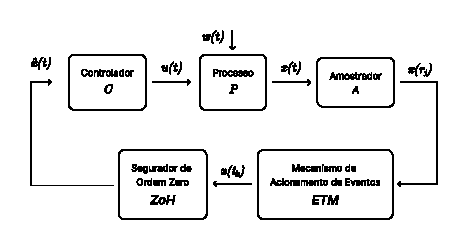
\includegraphics[scale=2.]{figuras/etc-model.eps}
  \caption{Modelo de um sistema dinâmico em loop fechado com ETC.}
  \label{fig:etc-model}
\end{figure}

% ETC: Estrutura
O modelo apresentado na \autoref{fig:etc-model} consiste em uma planta $ P$ que recebe uma entrada de perturbação não controlada $w(t)$ e a entrada de controle $u(t)$, e cujo estado é determinado por uma equação diferencial \begin{equation}\dot{x}(t) = f(x(t), u(t), w(t))\end{equation} A informação do estado pode ser monitorada de forma contínua ou amostrada, o que caracteriza o \acrshort{etc} como contínuo ou periódico, respectivamente. No caso do \acrshort{etc} periódico, um sistema de amostragem é introduzido para gerar uma sequência discreta de estados $x(t_A)$, onde o $t_A$ é o tempo de liberação do estado medido. Por outro lado, no \acrshort{etc} contínuo, o estado medido é enviado diretamente para o \acrshort{etm}. \cite{peng2018,coutinho2021,Lemmon2010}.

% ETC: Função do ETM e comportamento Zeno
O \acrshort{etm} determina o instante apropriado para transmitir o estado para o \acrfull{zoh} - que é utilizado para transformar o sinal discreto resultante em um sinal contínuo no tempo,  para estar disponível para o controlador $C$ que irá mapear esses estados amostrados em um sinal de controle e aplicar à planta. \cite{coutinho2021}. Para garantir a eficácia do \acrshort{etm}, é crucial evitar o comportamento Zeno. Esse comportamento ocorre quando o controlador executa uma quantidade infinita de tarefas de controle dentro de um intervalo de tempo finito, contrariando a premissa fundamental do \acrshort{etc} de minimizar os tempos de execução de tarefas. Além disso, o fenômeno de Zeno exerce uma considerável influência nos comportamentos dinâmicos dos sistemas, manifestando-se em instabilidade, degradação de desempenho e oscilações indesejadas. \cite{Yang2024}.

% ETC: Diferentes Abordagens - Introdução e Abordagem por Emulação
O projeto eficiente tanto do \acrshort{etm} quanto das leis de controle é crucial para assegurar o desempenho adequado e a estabilidade dos sistemas \acrshort{etc} em malha fechada. Como resultado, os modelos de \acrshort{etc} frequentemente adotam abordagens baseadas em emulação ou co-design para atingir tais objetivos. \cite{coutinho2021, peng2018}. As abordagens baseadas em emulação são geralmente realizadas em dois passos distintos. Primeiramente, um controlador é projetado para garantir a estabilidade ou um desempenho específico para o sistema em malha fechada, assumindo a ausência do \acrshort{etm} e da rede de comunicação. Este controle é projetado de acordo com uma estrutura convencional de dados amostrados periódicos, aproveitando os resultados proveitosos dos sistemas de dados amostrados. \cite{coutinho2021,peng2018}. Em seguida, o segundo passo envolve a consideração da presença do \acrshort{etm} e dos efeitos induzidos pela rede de comunicação, a fim de projetar o \acrshort{etm} de forma a preservar as propriedades garantidas pelo controlador previamente projetado. Esta abordagem permite que o \acrshort{etm} seja projetado separadamente do controle, conferindo flexibilidade no processo de projeto. \cite{coutinho2021,peng2018}. No entanto, essa independência pode limitar o desempenho em malha fechada do sistema \acrshort{etc} e exigir mais transmissões do que o necessário, uma vez que o \acrshort{etm} pode não estar otimizado para o controle específico. \cite{coutinho2021}.

% ETC: Diferentes Abordagens - Abordagem por Co-design
As abordagens baseados no \textit{co-design} buscam superar as limitações das abordagens baseadas em emulação, permitindo o design simultâneo do \acrshort{etm} e da lei de controle. No entanto, o \textit{co-design} enfrenta desafios como problemas de otimização não-convexos ou multiobjetivo, devido a restrições conflitantes de desempenho e aumento dos tempos entre eventos. A análise muitas vezes se limita a classes específicas de controladores e \acrshortpl{etm} \cite{coutinho2021}. Diferentes estratégias de \textit{co-design} têm sido desenvolvidas para várias formas de \acrshortpl{etm}. Estas incluem \textit{co-design} estático para estabilização local de sistemas LTI e \textit{co-design} dinâmico para sistemas lineares com entradas não lineares limitadas, entre outros. As condições de \textit{co-design} são frequentemente derivadas usando formalismos de sistema híbrido e expressas em termos de \acrshortpl{lmi}, permitindo uma eficiente resolução por métodos de otimização convexa \cite{coutinho2021}.

% ETC: ETM estático e dinâmico (adaptativa)
Os modelos de \acrshort{etm} podem ser diferenciados em termos da lei de acionamento, que pode ser estática ou adaptativa (dinâmica). No contexto do \acrshort{etm} estático, os instantes de transmissão são determinados com base em uma função de acionamento estática. Destaca-se, a título de ilustração, o \acrshort{etc} contínuo estático proposto por Tabuada \cite{Tabuada2007}, esclarecendo sua eficácia para sistemas não lineares em malha fechada, onde a estabilidade é garantida por meio de uma função \acrfull{ees} de \textit{Lyapunov}.

Para reduzir o número de eventos transmitidos, foram propostas funções de acionamento aprimoradas \cite{Wang2020,Zong2023,Ge2017, Ning2018, Wu2021}, introduzindo variáveis dinâmicas. Uma alternativa é considerar uma função de ponderação variável no tempo, caracterizando o \acrshort{etc} adaptativo ou dinâmico, desenvolvido principalmente no contexto de sistemas \acrshort{etc} periódico \cite{coutinho2021}. Este método permite ajustar dinamicamente o limite de acionamento, proporcionando uma adaptação mais flexível às condições do sistema. A estabilidade do sistema sob o \acrshort{etc} adaptativo é analisada usando uma função de \textit{Lyapunov} modificada, demonstrando sua eficácia em manter a estabilidade em malha fechada \cite{coutinho2021}.

% ETC: Rede de Comunicação
Os efeitos induzidos aos estados transmitidos pela rede de comunicação $\mathcal{N}$ são de suma importância e têm um impacto direto na estabilidade e no desempenho do sistema. Quando os estados são transmitidos por meio da rede, podem surgir distorções e atrasos devido a vários fatores, como variações nos intervalos de transmissão, atrasos na própria rede e possíveis perdas de pacotes. Essas perturbações nos estados transmitidos podem resultar em erros na estimativa do estado real no controlador, afetando diretamente a capacidade do sistema de alcançar os objetivos de controle desejados. Assim, é essencial compreender e mitigar esses efeitos nos estados transmitidos para garantir um projeto eficaz dos controladores, o que por sua vez assegura a estabilidade e o desempenho adequados do sistema em malha fechada. \cite{coutinho2021}.

% ETC: Conclusão
As diferentes abordagem de \acrshort{etc} abrangem investigações em controladores de retroalimentação de estado, observadores, \acrshortpl{etm} estáticos e dinâmicos, com o intuito de assegurar a estabilidade e o desempenho em malha fechada em uma variedade de sistemas, tais como sistemas \acrfullpl{lit} \cite{Zong2023,Wu2021}, sistemas de \textit{Lur'e} \cite{Zhang2017} e modelos \textit{fuzzy Takagi-Sugeno} \cite{Pan2017}. O foco está em estabelecer condições práticas e numericamente solucionáveis que simplifiquem o projeto eficaz de sistemas de controle complexos.

% ---------------------------------------------------------------------------
\section{\acrshort{etm} Dinâmico e Estático}

% ETM: Apresentação do trabalho de Coutinho
Em sua pesquisa, Coutinho investigou um modelo de \acrshort{etm} dinâmico e estático, sobre o qual este projeto se fundamenta. Este modelo baseia-se em uma condição suficiente para permitir o projeto simultâneo do \acrshort{etm} e do controlador com ganhos escalonados, por meio da abordagem por co-design, garantindo a estabilidade assintótica da origem do sistema em malha fechada. Além disso, ele provou a existência de um \acrfull{imee} positivo que evita a existência de comportamento de Zeno a fim de garantir sua aplicabilidade, pois as redes de comunicação não têm largura de banda infinita para suportar tempos entre eventos arbitrariamente próximos. Por fim, aborda um problema de otimização visando a ampliação dos intervalos entre eventos, com o objetivo de minimizar a quantidade de eventos gerados pelo \acrshort{etm}. \cite{coutinho2021}.

% ETM: Apresentação do sistema dinâmico
O modelo proposto por Coutinho para o \acrshort{etm} dinâmico considera uma classe específica de sistemas não lineares, representada pela equação diferencial abaixo: \begin{equation} \dot{x}(t) = A(x(t))x(t) + B(x(t))u(t). \label{eq:etm-sys}\end{equation} Nesta equação, $ x(t) \in D \subset \mathbb{R}^n $ representa o estado do sistema, $ u(t) \in \mathbb{R}^m $ é a entrada de controle, e $ A: D \rightarrow \mathbb{R}^{n \times n} $ e $ B: D \rightarrow \mathbb{R}^{n \times m} $ são funções contínuas de matriz, com a restrição de que $ B(x) \neq 0 $ para todo $ x \in D $. Os termos não lineares nos coeficientes dependentes do estado, $ A(x) $ e $ B(x) $, são representados por $ z_j: D \rightarrow \mathbb{R} $, onde $ j \in \mathbb{N}_{\leq p} $, e são denominados funções de escalonamento. Aqui, $ D \subset \mathbb{R}^n $ é um politopo convexo que inclui a origem, sendo esta considerada o ponto de equilíbrio de interesse. \cite{coutinho2021}.

% Definição das funções de escalonamento e de ponderamento
% Warning Este texto é praticamente igual a do Coutinho
Dado que as funções de escalonamento $z_j(x)$ são contínuas e $D$ é um conjunto compacto, podemos inferir a existência de limites, de forma que: \begin{equation} z_{j}^0 \leq z_j(x) \leq z_{j}^0, \quad \forall j \in \mathbb{N}_{\leq p}. \end{equation} Assim, cada função de escalonamento $z_j(x)$ pode ser representada de maneira equivalente como: \begin{equation} z_j(x) = w_0^j(x)z_j^0 + w_{1}^j(x)z_{j}^1 = \sum_{i_j=0}^{1} w_{i_j}^j(x)z_i^{i_j}, \end{equation} onde as funções de ponderação dependentes do estado são definidas como: \begin{equation} w_0^j(x) := \frac{z_j^1 - z_j(x)}{z_j^1 - z_j^0}, \quad w_1^j(x) := 1 - w_0^j(x), \end{equation} com $0 \leq w_i^j(x) \leq 1$, $i_j \in \mathbb{B}$, $j \in \mathbb{N}_{\leq p}$. Portanto, para todo $x \in D$, o sistema não linear \eqref{eq:etm-sys} pode ser equivalente ao seguinte modelo quasi-LPV poliédrico: \begin{equation} \dot{x}(t) = \sum_{i \in \mathbb{B}_p} w_i(x(t))(A_i x(t) + B_i u(t)), \label{eq:etm-politopic} \end{equation} onde os parâmetros dependentes do estado são definidos como: \begin{equation} w_i(x) := \prod_{j=1}^{p} w_{ij}^j(x), \end{equation} sendo $i = (i_1, ..., i_p) \in \mathbb{B}_p$. Por definição, observamos que a propriedade de soma convexa permanece válida para os parâmetros: \begin{equation} \sum_{i \in \mathbb{B}_p} w_i(x) = 1, \quad 0 \leq w_i(x) \leq 1, \quad \forall i \in \mathbb{B}_p, \end{equation} garantindo que as matrizes: \begin{equation} \left. A_i := A(x) \right|_{w_i(x)=1}, \quad \left.B_i := B(x) \right|_{w_i(x)=1}, \end{equation} definem os vértices do modelo quasi-LPV poliédrico \eqref{eq:etm-politopic}. \cite{coutinho2021}.

% ETM: Lei de controle 
A seguinte lei de controle de realimentação de estado, com ganhos escalonados, é considerada para estabilizar o sistema \eqref{eq:etm-sys}:
\begin{equation} u(t) = K(\hat{x}(t))\hat{x}(t) = \sum_{j \in Bp} w_j(\hat{x}(t))K_j\hat{x}(t) \end{equation} onde $ \hat{x}(t) $ representa a informação de estado disponível para o controlador através do ETM. A matriz dependente de estado $ K : D \rightarrow \mathbb{R}^{m \times n} $ é assumida como dependente das funções de escalonamento de \eqref{eq:etm-sys}, de modo que um controlador programado para ganho com ganhos $ K_j = K(\hat{x}) $ possa ser parametrizado em termos dos parâmetros $ w_j(\hat{x}) $. \cite{coutinho2021}.

% ETM: Apresentação do erro de transmissão
Quando uma amostra de dados é transmitida no tempo do evento $t_k$, o estado disponível para o controlador é atualizado para $\hat{x}(t) = x(t_k)$, para todo $t \in [t_k, t_{k+1})$. Como é utilizado um \acrshort{zoh}, $\hat{x}(t)$ é mantido constante até o próximo tempo de evento $t_{k+1}$, o que induz o erro de transmissão \begin{equation}e(t) = \hat{x}(t) - x(t) \label{eq:etm-error},\end{equation} $\forall t \in [t_k, t_{k+1})$. \cite{coutinho2021}.

% ETM: Tempo de ocorrência dos eventos e a variável interna dinâmica
O tempo de ocorrência dos eventos é determinado pela seguinte equação: \begin{equation} t_0 = 0, t_{k+1} = \inf \{t > t_k : \eta(t) + \theta \Gamma(x(t), e(t) < 0) \}, \, \forall k \in \mathbb{N}, \end{equation} onde $\theta \in \mathbb{R}_{\geq 0}$ é um parâmetro de projeto e a função de acionamento $\Gamma(x, e)$ é definida como: \begin{equation} \label{eq:etm-gama} \Gamma(x, e) = x^T \Psi x - e^T \Xi e - \zeta (x,e), \end{equation} com \begin{equation} \zeta(x, e) = 2x^TPB(x)(K(\hat{x}) - K(x))(x+e). \end{equation} A dinâmica da variável interna do \acrshort{etm} é definida como: \begin{equation}  \dot{\eta} = - \lambda \eta(t) + \Gamma(x(t), e(t)), \end{equation} onde $\lambda \in R_{\geq} 0 $ é o parâmetro de projeto relacionado à taxa de decaimento de $\eta(t)$. \cite{coutinho2021}.

% ETM: Condições de Co-design

A condição suficiente proposta para projeto por co-design para o ETC contínuo  e o controlador por ganhos escalonados é declarada a seguir.
\begin{theorem}
  \label{theorem:constraints-2}
  Dados $\theta, \eta_0 \in \mathbb{R}_{\geq 0}$, e $\lambda \in \mathbb{R}_{> 0}$, se existirem as matrizes $\tilde{K}_j \in \mathbb{R}^{m \times n}, j \in B_p$. e matrizes simétricas positivas definidas $\Xi, \Psi, X \in \mathbb{R}$, satisfazendo as seguintes \acrshortpl{lmi}:
  \begin{equation}
    \sum_{(\mathbf{i}, \mathbf{j}) \in \mathscr{P} (\mathbf{m},\mathbf{n})} \Upsilon_{\mathbf{ij}} < 0, \quad \forall \mathbf{m}, \mathbf{n} \in B_p^+,
    \label{eq:2.18}
  \end{equation}
  onde
  \begin{equation}
    \Upsilon_{\mathbf{ij}} :=
    \begin{bmatrix}
      He(A_\mathbf{i}X +B_\mathbf{i}\tilde{K}_\mathbf{j}) & B_\mathbf{i}\tilde{K}_{\mathbf{j}} & X             \\
      \star                                               & -\tilde{\Xi}                       & 0             \\
      \star                                               & \star                              & -\tilde{\Psi}
    \end{bmatrix},
  \end{equation}
  então, a origem do sistema de malha fechada é assintoticamente estável com $K_j = \tilde{K}_jX^{-1}$, $j \in B^p$, $\Xi= X^{-1}\tilde{\Xi}X$, $\Psi = \tilde{\Psi}^{-1}$, $P = X^{-1}$ e função de Lyapunov
  \begin{equation}
    W(x, \eta) = V(x) + \eta,
  \end{equation}
  com $V(x)=x^TPx$.
\end{theorem}

Para reduzir o número de eventos gerados, Coutinho propôs o seguinte problema de otimização convexa que visa minimizar $\lambda_{\max} (\Xi)$ e maximizar $\lambda_{\min}(\Psi)$: \begin{equation}\underset{Q, X, \tilde{\Xi}, \tilde{\Psi}, \tilde{K}_\mathbf{j}}\min \quad \mathbf{tr}(\tilde{\Xi} + \tilde{\Psi} + Q).\end{equation} Este problema é sujeito a restrições apresentadas no \autoref{theorem:constraints-2} e à seguinte \acrshort{lmi} de restrição \begin{equation}\begin{bmatrix}
  -Q & I \\ \star & -X
\end{bmatrix} < 0.\end{equation} A solução deste problema tende a minimizar os autovalores de $Q$, $\tilde{\Xi}$ e $\tilde{\Psi}$ e a reduzir os tempos entre os eventos. \cite{coutinho2021}.

Ao considerar um valor de $\theta$ suficientemente grande, o \acrshort{etm} dinâmico converge para uma versão estática, que se torna completamente independente de $\eta(t)$, conforme descrito a seguir: \begin{equation} t_0 = 0, \quad t_{k+1} = \inf\{t > t_k : \Gamma(x, e) < 0\}, \forall k \in \mathbb{N}, \end{equation} onde $\Gamma(x, e)$ é definido em \eqref{eq:etm-gama}. \cite{coutinho2021}.

\section{Trabalhos Relacionados}

A área de sistemas \acrshort{etc} já possui diversas técnicas estabelecidas que têm demonstrado resultados promissores. As estratégias adotadas neste projeto têm sua base em pesquisas destacadas que serão apresentadas a seguir

% To-do: Explicar sobre o comportamento Zeno na fundamentação
% Dúvida: É para ser mais detalhistas em cada trabalho?
No estudo realizado por Coutinho \cite{coutinho2021}, é investigado o \textit{co-design} de controladores de retroalimentação de estado, e \acrshortpl{etm} contínuos e dinâmicos para sistemas comutados não lineares representados por modelos \textit{quasi} \acrfullpl{lpv}. A condição de \textit{co-design} é derivada com base na teoria da estabilidade de \textit{Lyapunov} para garantir a estabilidade assintótica do sistema \textit{Lyapunov} em malha fechada. Para lidar com o fenômeno assíncrono entre o controlador e os parâmetros do modelo \textit{quasi}-\acrshort{lpv} induzido pela ação do \acrshort{etm}, é proposta uma função de acionamento que cancela essa influência, resultando em uma condição de \textit{co-design} menos conservadora. Também é introduzido um problema de otimização convexa para aumentar os tempos entre eventos. Ademais, é demonstrada a existência de um \acrfull{imee} para o \textit{etc} contínuo proposto, evitando o comportamento \textit{Zeno}. Além disso, são apresentadas as vantagens da abordagem de \textit{co-design} dinâmico sobre a abordagem baseada em emulação e sua versão estática.

% Lembrete: Este trabalho apresenta a definição de zoh
% Dúvida: Há um termo melhor para 'switched systems'?
\textit{Ren et al}. \cite{Ren2018} abordaram o controle resiliente de tempo finito com base em observadores para sistemas comutados, realizado em um \acrfull{ecae}. Diferenciando-se dos problemas tradicionais de tempo finito, este estudo considera não apenas o \acrfull{ltf}, mas também a \acrfull{efes}. Um \acrshort{ecae} é formulado para sistemas comutados, visando uma utilização eficiente dos recursos da rede. Para lidar com a impossibilidade de medir todos os estados, é desenvolvido um observador acionado por eventos, que serve como base para a construção de um controlador resiliente. Esse controlador demonstra robustez ao estabilizar os sistemas em questão, dentro do contexto do controle de tempo finito. Utilizando o método de atraso no tempo e a abordagem de \textit{Lyapunov}, são derivados resultados significativos para avaliar as propriedades dos \acrshortpl{ltf} e da \acrshort{efes} dos sistemas de erro comutados em circuito fechado acionados por eventos. Todas as desigualdades matriciais são transformadas em \acrshortpl{lmi} para facilitar a obtenção conjunta dos ganhos do controlador e do observador. Por fim, a eficácia do esquema de controle proposto é demonstrada através de sua aplicação em um sistema de circuito de conversor \textit{boost}.

No estudo apresentado por \textit{Soni et al}. \cite{Soni2023}, é proposto o \acrshort{etc} para o modelo \acrshort{lpv} de conversores \textit{boost}. O controlador proposto, dependente da razão de ciclo, demonstra melhor desempenho e menor demanda computacional. Utilizando a função de \textit{Lyapunov } dependente de parâmetros, foi realizada a análise de estabilidade da abordagem proposta. Além disso, é estabelecido que o tempo entre eventos é limitado inferiormente por uma constante positiva, assegurando um desempenho livre de comportamento \textit{Zeno}. Os resultados de simulação e experimentais deste estudo validam a eficácia do método proposto, evidenciando que o modelo proporciona desempenho e maior robustez.

% Dúvida: Há um termo melhor para 'switched systems'?
No estudo realizado por Ma et al. \cite{Ma2016}, o problema do \acrshort{etc} com base em retroalimentação de saída para sistemas lineares comutados é investigado. Os autores projetam um controlador acionado por eventos e derivam condições suficientes para garantir a estabilidade assintótica do sistema comutado, utilizando métodos da função de \textit{Lyapunov} e técnicas de \acrshortpl{lmi}. Além disso, eles demonstram que o \acrshort{imee} acionados é positivo, eliminando o comportamento Zeno na amostragem. Por fim, os pesquisadores aplicam seu método a sistemas comutados de conversores \textit{boost} para validar sua eficácia.

\textit{Xie et al.} \cite{Xie2023} abordam os problemas da análise de \acrshort{efes} e do projeto de controlador de retroalimentação de saída para sistemas afins comutados sujeitos a perturbações externas. Um observador afim comutado é desenvolvido para estimar estados não mensuráveis, seguido pela proposição de um \acrshort{etm} dinâmico capaz de evitar o comportamento Zeno e reduz a carga de transmissão da rede. As condições viáveis da \acrshort{ees} são apresentadas em formas de \acrshortpl{lmi}, baseadas em uma função de \textit{Lyapunov-Krasovskii} temporal e leis de comutação dependentes do estado. A eficácia do algoritmo proposto é demonstrada através de um exemplo de aplicação com um conversor \textit{flyback} CC-CC.

No artigo \cite{Kumar2020}, Kumar et al. introduzem um novo conceito de \acrshort{etc} para otimizar o uso de recursos em \acrshort{mgcc}. Um \acrfull{cmd} é combinado com um observador de perturbações integral para suprimir incertezas combinadas e não combinadas em modo conectado à rede e isolado. O controlador resultante regula a tensão do barramento \acrshort{cc} e melhora a estabilidade operacional da \acrshort{mr}. Um \acrshort{cmd} convergente em tempo finito, livre de oscilações, é desenvolvido com uma lei de alcance de super torção para garantir robustez. A eficácia do \acrshort{etc} é comparada com abordagens alternativas e demonstrou um desempenho superior.

\chapter{Conversores CC com Cargas de Potência Constante} \label{cap3}

\section{Microrredes CC}

No século XX, a "Guerra das Correntes" entre defensores da \acrshortpl{ca}, liderados por \textit{Westinghouse} e \textit{Tesla}, e proponentes da \acrshort{cc}, liderados por \textit{Edison}, resultou na prevalência da \acrshort{ca} devido à sua facilidade de expansão da rede. Apesar disso, a \acrshort{cc} permaneceu relevante com os avanços na eletrônica de potência. Paralelamente, a crescente adoção de microrredes \acrshortpl{mr}, com \acrfullpl{fer}, \acrfullpl{sae} e novas cargas, reflete preocupações ambientais e escassez de combustíveis fósseis, mas sua integração descoordenada apresenta desafios técnicos e operacionais, como perfil de tensão comprometido e congestionamentos nas linhas de transmissão. \cite{Elsayed2015, Dragicevic2015}.

A proposta das \acrshortpl{mr} surgiu como uma solução há mais de uma década. As \acrshortpl{mr}, operando em modo isolado ou conectadas à rede, podem ser classificadas como \acrshortpl{mr} de \acrshort{ca} ou \acrshort{cc}, sendo a \acrshort{mr} de \acrshort{cc} mais atraente devido à sua maior eficiência e melhor interface com diversos tipos de \acrshort{fer} e \acrshort{sae}. Além disso, ao serem acopladas em torno de um barramento \acrshort{cc}, as \acrfullpl{mr} eliminam problemas como fluxo de potência reativa e regulação de frequência, resultando em sistemas de controle menos complexos. \cite{Dragicevic2015}.

Vários setores empregam \acrfullpl{sdcc}, como espaçonaves, centros de dados, telecomunicações, tração e sistemas de energia a bordo de navios. Por exemplo, a Estação Espacial Internacional utiliza \acrshortpl{sdcc} para operar suas vastas necessidades de energia. Alguns centros de dados também adotaram sistemas \acrshort{cc}, resultando em economia significativa de energia em comparação com sistemas \acrshort{ca} tradicionais. Na área de telecomunicações, os sistemas de distribuição de energia de 48V são amplamente empregados para garantir alta confiabilidade e eficiência. Além disso, sistemas de tração, como bondes e metrôs, preferem distribuição \acrshort{cc} devido à facilidade de interface com motores \acrshort{cc}. Esses sistemas também permitem maior eficiência e controlabilidade. Em sistemas de energia a bordo de navios, a distribuição zonal \acrshort{cc} é uma opção popular devido à sua confiabilidade e facilidade de proteção. \cite{Elsayed2015}.

Desta forma, o design de sistemas de distribuição \acrshort{cc} tem recebido atenção crescente, especialmente devido a adaptação de equipamentos projetados originalmente para \acrshort{ca}. Modelos simplificados são essenciais para compreender o comportamento da carga em operação \acrshort{cc}. Comparando configurações de cabos, descobriu-se que sistemas \acrshort{cc} podem superar \acrshort{cc} em termos de capacidade de transferência de energia, \cite{Salomonsson2007}. Em um estudo sobre microrredes \acrshort{cc} em centros de dados, \cite{Salomonsson2008}, foi proposto um sistema de controle adaptativo para otimizar o fluxo de energia e minimizar perdas. A coordenação entre conversores é crucial para garantir o fornecimento contínuo de energia às cargas sensíveis. Essas pesquisas contribuem para uma compreensão mais profunda do design e controle de sistemas de distribuição DC.

\section{Conversores CC e Cargas de Potência Constante}



\section{Modelagem Matemática}

% Introdução
% To-do: não esquecer de apresentar a forma completa da CPL
Nesta seção, aprofundaremos na modelagem matemática de uma microrrede, concentrando em um conversor buck operando em conjunto com uma \acrshort{cpl}. O conversor buck assume um papel fundamental na conversão de alta para baixa tensão contínua, enquanto a \acrshort{cpl} representa um tipo de carga com uma demanda de potência invariável, mesmo diante de flutuações na tensão de entrada. Essa análise aprofundada tem como objetivo desvendar os princípios basilares que regem essa configuração específica da microrrede, lançando as bases para análises subsequentes e o desenvolvimento de estratégias de controle eficazes.

Para facilitar cálculos e análises, este sistema simplificado será composta por um conversor buck e a \acrshort{cpl} será modelada como uma fonte de corrente, como apresentado na \autoref{fig:circuit1}. Essa modelagem captura o comportamento essencial que permite o estudo aprofundado das estratégias de \acrshort{etc} para conversores \acrshort{cc}. No circuito apresentado, os componentes incluem resistores ($R_L$, $R_C$), um capacitor ($C$) e um indutor ($L$). O parâmetro $d$ representa o \textit{duty cycle}, enquanto $I_{\acrshort{cpl}}$ indica a corrente da \acrshort{cpl}. Além disso, são observadas as tensões de entrada ($V_{in}$) e saída ($V_{out}$). Esses elementos desempenham papéis essenciais na operação e caracterização do circuito em questão, contribuindo para a compreensão abrangente de seu funcionamento e comportamento.

\begin{figure}[H]
  \centering
  % \vspace{3ex}
  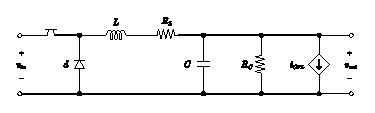
\includegraphics[scale=2.5]{figuras/buck_conversor_with_cpl_circuit.eps}
  \caption{Circuito \textit{Buck} com \acrshort{cpl}.}
  \label{fig:circuit1}
\end{figure}

% Introdução para o desenvolvimento das equações
% To-do: não esquecer de apresentar a forma completa do MMS e do MPS
% Dúvida: É para ser mais detalhista na obtenção das equações?
As equações que regem o comportamento do sistema são derivadas das leis fundamentais da eletricidade. O modelo matemático do conversor \textit{buck} se baseia no \acrshort{mms}. Apesar da natureza não linear intrínseca dos conversores, a prática usual é empregar \acrshort{mps} para obter uma representação linearizada em torno do ponto de operação. Para tal, o circuito é analisado em duas situações distintas: chave fechada e chave aberta.

% Modelagem do sistema para chave fechada
Na situação em que a chave está fechada, o circuito pode ser simplificado para um circuito série composto por uma fonte de tensão, um resistor e uma indutância, como ilustrado na \autoref{fig:circuit2}.

\begin{figure}[H]
  \centering
  % \vspace{3ex}
  \includegraphics[scale=2.5]{figuras/buck_conversor_with_cpl_circuit_m1.eps}
  \caption{Circuito com a chave fechada.}
  \label{fig:circuit2}
\end{figure}

\noindent As equações que descrevem esse circuito são apresentadas abaixo:
% Lembrança: Faltou explica o que seria a Pcpl

\begin{equation}
  \begin{cases}
    \frac{d}{dt}i_L =  \frac{1}{L} V_{in}  - \frac{R_L}{L} i_L - \frac{1}{L} v_C \\
    \frac{d}{dt} v_C = \frac{1}{C} i_L - \frac{1}{C R_C} v_C - \frac{1}{C v_C} P_{CPL}
    \label{eq:circuito-m1}
  \end{cases}
\end{equation}
\\
\indent Na segunda situação, a chave está aberta e, consequentemente, a fonte de tensão é desconectada do circuito. Essa situação é representada na \autoref{fig:circuit3}.

\begin{figure}[H]
  \centering
  % \vspace{3ex}
  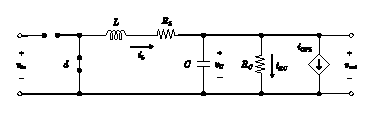
\includegraphics[scale=2.5]{figuras/buck_conversor_with_cpl_circuit_m2.eps}
  \caption{Circuito com a chave aberta.}
  \label{fig:circuit3}
\end{figure}

Neste caso, as equações que descrevem o circuito quando a chave está aberta são:

\begin{equation}
  \begin{cases}
    \frac{d}{dt}i_L  & = \frac{V_{in}}{L} d - \frac{R_L}{L} i_L - \frac{1}{L} v_C        \\
    \frac{d}{dt} v_C & = \frac{1}{C} i_L - \frac{1}{C R_C} v_C - \frac{1}{C v_C} P_{CPL}
    \label{eq:circuito-m2}
  \end{cases}
\end{equation}
\\
A partir da \autoref{eq:circuito-m1} e \autoref{eq:circuito-m2}, derivadas anteriormente, podemos estabelecer as seguintes equações diferenciais, as quais caracterizam o \acrshort{mms} e fornecem uma descrição do comportamento do circuito durante a operação contínua da chave.

\begin{equation}
  \begin{cases}
    \frac{d}{dt}i_L  & = \frac{V_{in}}{L} d - \frac{R_L}{L} i_L - \frac{1}{L} v_C        \\
    \frac{d}{dt} v_C & = \frac{1}{C} i_L - \frac{1}{C R_C} v_C - \frac{1}{C v_C} P_{CPL}
    \label{eq:nonlinear-system}
  \end{cases}
\end{equation}
\\
\indent Por meio da \autoref{eq:nonlinear-system}, onde é apresentado o sistema não linear, pode-se obter o sistema linearizado em torno dos pontos de operação. Esse sistema linear é representado por um conjunto de equações diferenciais, que descrevem as variações no tempo das grandezas $\delta i_L$ e $\delta v_C$, representando as alterações na corrente do indutor e na tensão do capacitor, respectivamente.

Considerando o sistema linearizado descrito por: \begin{equation} \dot{x} = Ax(t) + B_uu(t) + B_ww(t), \end{equation} onde  $x = \begin{bmatrix} \delta i_L & \delta v_C \end{bmatrix} ^ T$ representa o estado do sistema, $u = \delta d$ é a entrada do sistema e $w = \delta P_{CPL}$ é o sinal de pertubação. Além disto, $A \in \mathbb{R}^{n \times n}$, $B_u \text{ e } B_w \in \mathbb{R}^{n \times 1}$, são obtidos por meio das matrizes jacobianas das equações em (\ref{eq:nonlinear-system}), em torno do ponto de equilíbrio $P_{eq} = ({i_L}_0, \hspace{0.07cm} {v_C}_0, \hspace{0.07cm} {d}_0, \hspace{0.07cm} {P_{CPL}}_0)$. Portanto, o sistema linearizado obtido pode ser expresso como:

\begin{equation}
  \begin{bmatrix}
    \dot{\delta i_L} \\ \dot{\delta v_C}
  \end{bmatrix}
  =
  \begin{bmatrix}
    -\frac{R_L}{L} & -\frac{1}{L}                                                                \\
    \frac{1}{C}    & \frac{1}{C}\left(\frac{{P_{CPL}}_0}{{{{v_{C}}_0}^2}} - \frac{1}{R_C}\right)
  \end{bmatrix}
  \begin{bmatrix}
    \delta i_L \\ \delta v_C
  \end{bmatrix}
  +
  \begin{bmatrix}
    {\frac{V_{in}}{L}} & 0                     \\
    0                  & {-\frac{1}{C{v_C}_0}}
  \end{bmatrix}
  \begin{bmatrix}
    \delta d \\ \delta P_{CPL}
  \end{bmatrix}
\end{equation}

\section{Simulação}

\chapter{Controle Baseado em Eventos de Conversores CC-CC} \label{cap4}

% Essa análise fornece insights sobre a aplicação das abordagens de ETC e permite comparar suas vantagens e desvantagens.


\section{Modelo de \acrshort{etm} para Sistemas Lineares}

% ETM: Apresentação do sistema dinâmico
Nesta pesquisa, é proposto um modelo de \acrshort{etm} dinâmico para sistemas lineares, representada pela equação diferencial abaixo: \begin{equation} \dot{x}(t) = Ax(t) + Bu(t). \label{eq:linear_system_etm}\end{equation} Nesta equação, $ x(t) \in \mathbb{R}^n $ representa o estado do sistema, $ u(t) \in \mathbb{R}^m $ é a entrada de controle, e $ A \in \mathbb{R}^{n \times n} $ e $ B \in \mathbb{R}^{n \times m}$ são a matriz de estados e a matriz de entrada, respectivamente. Além disto, a origem do sistema é considerada o ponto de equilíbrio de interesse.

% ETM: Apresentação do erro de transmissão
Como discutido na seção \ref{section:etm_classification}, quando uma amostra de dados é transmitida no tempo de evento $t_k$, o estado disponível para o controlador é atualizado para $\hat{x}(t) = x(t_k)$, para todo $t$ no intervalo $[t_k, t_{k+1})$. Ao utilizar um \acrshort{zoh}, $\hat{x}(t)$ é mantido constante até o próximo tempo de evento $t_{k+1}$, resultando no erro de transmissão representado por: \begin{equation}
  e(t) = \hat{x}(t) - x(t), \quad \forall t \in [t_k, t_{k+1}).
\end{equation} Este erro ocorre durante o intervalo de tempo entre eventos, $ [t_k, t_{k+1})$.

Desta forma, considerando a seguinte lei de controle por realimentação de estados, ou seja, $u(t) = K\hat{x}(t)$, onde $K \in \mathbb{R}^{1 \times n}$, o sistema linear dinâmico em malha fechada \eqref{eq:linear_system_etm} pode ser expresso pela seguinte equação dinâmica: \begin{gather}
  \dot{x}(t) = Ax(t) + BK\hat{x}(t) \notag \\[12pt]c
  \dot{x}(t) = Ax(t) + BK[x(t) + e(t)] \notag \\[12pt]
  \dot{x}(t) = (A + BK)x(t) + BKe(t)
  \label{eq:etm_closed_loop}
\end{gather}


% Adicionar um conclusão

\subsection{\acrshort{etm} Estático e Dinâmico}

% Resumo sobre o ETM estático
Conforme apresentado anteriormente, o \acrshort{etm} estático opera considerando apenas os estados atuais do sistema $x(t)$ e o erro de transmissão $e(t)$, e a sua lei de acionamento de eventos é definida como: \begin{equation} t_0 = 0, t_{k+1} = \inf \{t > t_k : \Gamma(x(t), e(t)) < 0 \}, \, \forall k \in \mathbb{N}, \label{eq:static_etm}\end{equation} onde $\Gamma(x, e)$ representa a função de acionamento do \acrshort{etm}. Adicionalmente, para uma classe específica de funções $\Gamma$ dada por \begin{equation}
  \Gamma(x(t), e(t)) = \sigma \alpha(\|x(t)\|) - \beta(\|e(t)\|),
\end{equation} com $\sigma \in (0,1)$, o sistema em malha fechada é assintoticamente estável.

% Função evento proposta
Baseado nisso, é proposta uma condição suficiente para o projeto de um \acrshort{etm} estático e dinâmico usando a abordagem de co-design para o sistema dinâmico linear \eqref{eq:linear_system_etm} controlado por realimentação de estados. Para isso, é considerada uma função de acionamento tal que $\alpha(\|x(t)\|) = x^T(t)\Psi x(t)$, $\beta(\|e(t)\|) = e^T(t)\Xi e(t)$ e $\sigma = 1$, ou seja:  \begin{equation}
  \Gamma(x(t), e(t)) = x^T(t)\Psi x(t) - e^T(t)\Xi e(t),
  \label{eq:etm_gamma}
\end{equation}  onde $\Psi, \, \Xi \in \mathbb{R}^{n \times n}$, e a formulação do seguinte teorema:

\begin{theorem}
  \label{theorem:etm_stability}
  Se existirem matrizes semidefinidas positivas $\Xi, \Psi, X \in \mathbb{R}$ e uma matriz $\tilde{K} \in \mathbb{R}^{m \times n}$ que satisfaçam a seguinte \acrshort{lmi}:
  \begin{equation}
    \begin{bmatrix}
      \mathsf{He}(AX +B\tilde{K}) & B\tilde{K}   & X             \\
      \star                       & -\tilde{\Xi} & 0             \\
      \star                       & \star        & -\tilde{\Psi}
    \end{bmatrix} < 0,
    \label{eq:etm_lmi_1}
  \end{equation}
  então, a origem do sistema em malha fechada é assintoticamente estável com $K = \tilde{K}X^{-1}$, $\Xi= X^{-1}\tilde{\Xi}X^{-1}$, $\Psi = \tilde{\Psi}^{-1}$, $P = X^{-1}$ e a função de Lyapunov definida por $V(x)=x^TPx$.
\end{theorem}

\noindent \textit{Demostração.} Considere que a \acrshort{lmi} \eqref{eq:etm_lmi_1} é factível. Desde que $X$ seja uma matriz semidefinida positiva não singular, esta \acrshort{lmi} pode ser multiplicada por $\mathsf{diag}(X^{-1}, X^{-1}, I)$ no lado esquerdo e direito. Assim, \begin{gather}
  \begin{bmatrix}
    X^{-1} & 0      & 0 \\
    0      & X^{-1} & 0 \\
    0      & 0      & I
  \end{bmatrix}
  \begin{bmatrix}
    \mathsf{He}(AX +B\tilde{K}) & B\tilde{K}   & X             \\
    \star                       & -\tilde{\Xi} & 0             \\
    \star                       & \star        & -\tilde{\Psi}
  \end{bmatrix}
  \begin{bmatrix}
    X^{-1} & 0      & 0 \\
    0      & X^{-1} & 0 \\
    0      & 0      & I
  \end{bmatrix}
  < 0, \notag \notag \\[12pt]
  \begin{bmatrix}
    \mathsf{He}(X^{-1}AX +X^{-1}B\tilde{K}) & X^{-1}B\tilde{K}   & I             \\
    \star                                   & -X^{-1}\tilde{\Xi} & 0             \\
    \star                                   & \star              & -\tilde{\Psi}
  \end{bmatrix}
  \begin{bmatrix}
    X^{-1} & 0      & 0 \\
    \star  & X^{-1} & 0 \\
    \star  & \star  & I
  \end{bmatrix}
  < 0, \notag \notag \\[12pt]
  \begin{bmatrix}
    \mathsf{He}(X^{-1}A +X^{-1}B\tilde{K}X^{-1}) & X^{-1}B\tilde{K}X^{-1}   & I             \\
    \star                                        & -X^{-1}\tilde{\Xi}X^{-1} & 0             \\
    \star                                        & \star                    & -\tilde{\Psi}
  \end{bmatrix}
  < 0,
\end{gather} Como $K = \tilde{K}X^{-1}$, $\Xi= X^{-1}\tilde{\Xi}X^{-1}$, $\Psi = \tilde{\Psi}^{-1}$, $P = X^{-1}$, têm-se: \begin{equation}
  \begin{bmatrix}
    \mathsf{He}(PA +PBK) & PBK   & I             \\
    \star                & -\Xi  & 0             \\
    \star                & \star & -\tilde{\Psi}
  \end{bmatrix} < 0
  \label{eq:inequation_prove}
\end{equation} Por meio do teorema de Schur, a inequação \eqref{eq:inequation_prove} pode ser reescrita como: \begin{equation}
  A_{\mathrm{S}} - B_{\mathrm{S}}D_{\mathrm{S}}^{-1}C_{\mathrm{S}} < 0,
\end{equation} onde, \begin{equation}
  A_{\mathrm{S}} = \begin{bmatrix}
    \mathsf{He}(PA +PBK) & PBK  \\
    (PBK)^T              & -\Xi
  \end{bmatrix}, \,
  B_{\mathrm{S}} = \begin{bmatrix}
    I \\ 0
  \end{bmatrix}, \,
  C_{\mathrm{S}} = \begin{bmatrix}
    I & 0
  \end{bmatrix} \, \mathrm{e} \,
  D_{\mathrm{S}} = -\tilde{\Psi}
\end{equation} Logo, \begin{gather}
  \begin{bmatrix}
    \mathsf{He}(PA +PBK) & PBK  \\
    \star                & -\Xi
  \end{bmatrix} -
  \begin{bmatrix}
    -\tilde{\Psi}^{-1} \\ 0
  \end{bmatrix}
  \begin{bmatrix}
    I & 0
  \end{bmatrix} < 0, \notag \notag \\[12pt]
  \begin{bmatrix}
    \mathsf{He}(PA +PBK) & PBK  \\
    \star                & -\Xi
  \end{bmatrix} -
  \begin{bmatrix}
    -\Psi & 0 \\ 0 & 0
  \end{bmatrix} < 0, \notag \notag \\[12pt]
  \begin{bmatrix}
    \mathsf{He}(PA + PBK) + \Psi & PBK  \\
    \star                        & -\Xi
  \end{bmatrix} < 0
  \label{eq:inequation_prove_2}
\end{gather} Multiplicando a inequação \eqref{eq:inequation_prove_2} por $\begin{bmatrix}
    x^T(t) & e^T(t)
  \end{bmatrix}$ no lado esquerdo, e por $\begin{bmatrix}
    x(t) & e(t)
  \end{bmatrix}^T$ no lado direito, obtém-se: \begin{gather}
  \begin{bmatrix}
    x^T(t) & e^T(t)
  \end{bmatrix}
  \begin{bmatrix}
    \mathsf{He}(PA + PBK) + \Psi & PBK  \\
    \star                        & -\Xi
  \end{bmatrix}
  \begin{bmatrix}
    x(t) \\ e(t)
  \end{bmatrix} < 0 \notag \\[12pt]
  \begin{bmatrix}
    x^T(t) (\mathsf{He}(P(A + BK)) + \Psi) + e^T(t) (PBK)^T &
    x^T(t) PBK - e^T(t) \Xi
  \end{bmatrix}
  \begin{bmatrix}
    x(t) \\ e(t)
  \end{bmatrix} < 0 \notag \\[12pt]
  x^T(t) (\mathsf{He}(P(A + BK)) + \Psi) x(t) + e^T(t) (PBK)^T x(t) +
  x^T(t) PBK e(t) - e(t)^T \Xi e(t)
  < 0 \notag \\[12pt]
  x^T(t) (P\mathsf{He}(A + BK) + \Psi) x(t) + e^T(t) (PBK)^T x(t) +
  x^T(t) PBK e(t) - e(t)^T \Xi e(t)
  < 0 \notag \\[12pt]
  2x^T(t) P[(A + BK)x(t) + BKe(t)] + x^T(t)\Psi x(t) - e^T(t) \Xi e(t)
  < 0
  \label{eq:inequation_prove_3}
\end{gather}  A partir das equações \eqref{eq:linear_system_etm} e \eqref{eq:etm_gamma}, a equação \eqref{eq:inequation_prove_3} pode ser reescrita como: \begin{gather}
  2x^T(t) P\dt{x}(t) + x^T(t)\Psi x(t) - e^T(t) \Xi e(t)  < 0 \notag \\[12pt]
  2x^T(t) P\dt{x}(t) + \Gamma(x(t), e(t)) < 0
  \label{eq:inequation_prove_4}
\end{gather} Como $2x^T(t) P\dt{x}(t) = x^T(t) P\dt{x}(t) + \dt{x}^T(t) P x(t)$ e $\Gamma(x, e) \geq 0, \, \forall t \in [t_k, t_{k+1}), \, \forall k \in \mathbb{N}$ então: \begin{equation}
  x^T(t) P\dt{x}(t) + \dt{x}^T P x(t)  < - \Gamma(x(t), e(t)) < 0.
\end{equation} Logo, \begin{equation}
  x^T(t) P\dt{x}(t) + \dt{x}^T(t) P x(t) < 0.
  \label{eq:final_inequation_prove}
\end{equation} Considerando a função de Lyapunov $V(x) = x^T(t)Px(t)$, a desigualdade \eqref{eq:final_inequation_prove} garante que $\dt{V}(x) < 0$. Portanto, a origem do sistema em malha fechada sob o \acrshort{etm} estático \eqref{eq:static_etm} é assintoticamente estável.

% ETM: Tempo de ocorrência dos eventos e a variável interna dinâmica
No \acrshort{etm} dinâmico, a lei de acionamento de eventos é definida como: \begin{equation} t_0 = 0, t_{k+1} = \inf \{t > t_k : \eta(t) + \theta \Gamma(x(t), e(t)) < 0 \}, \, \forall k \in \mathbb{N} \label{eq:dinamic_etm}\end{equation} onde $\theta \in \mathbb{R}_{\geq 0}$ é um parâmetro de projeto, a função de acionamento $\Gamma(x, e)$ é a mesma definida para o \acrshort{etm} estático, em \eqref{eq:etm_gamma} e $\eta$ é a variável dinâmica definida por: \begin{equation}  \dot{\eta} = - \lambda \eta(t) + \Gamma(x(t), e(t)), \label{eq:eta_dynamic}\end{equation} onde $\lambda \in R_{> 0} $ é o parâmetro de projeto relacionado à taxa de decaimento de $\eta(t)$.

Enquanto o \acrshort{etm} dinâmico não aciona um novo evento, têm-se $\eta(t) + \theta \Gamma(x(t), e(t)) \geq 0$. Se $\theta$ for nulo, então $\eta \geq 0$. Se $\theta$ não for nulo, então \begin{equation}
  \Gamma(x(t), e(t)) \geq - \frac{1}{\theta}\eta(t).
\end{equation} Logo, a partir de \eqref{eq:eta_dynamic},  \begin{equation}
  \dt{\eta}(t) \geq - \left(\lambda + \frac{1}{\theta}\right) \eta(t).
\end{equation} Assim, \begin{equation}
  \eta(t) \geq \eta(0) e ^ {-\left(\lambda + \frac{1}{\theta}\right) t}.
\end{equation} Portanto, $\eta(t) \geq 0$, para todo $t \in [t_k, t_{k+1}), \, \forall k \in \mathbb{N}$. Desta forma, têm-se que $\lambda \eta(t) \geq 0$ e, sob o \autoref{theorem:etm_stability}, a partir da equação \eqref{eq:inequation_prove_4} da demostração apresentada, obtém-se a seguinte inequação para o \acrshort{etm} dinâmico: \begin{gather}
  2x^T(t) P\dt{x}(t) + \Gamma(x(t), e(t)) - \lambda \eta(t) < 0 \notag \\[12pt]
  2x^T(t) P\dt{x}(t) + \dt{\eta}(t) < 0.
\end{gather} Do \autoref{theorem:etm_stability}, foi definido a seguinte função de Lyapunov $V(x) = x^TPx$, logo: \begin{equation}\dt{V}(x) = x^T(t)P\dt{x}(t) + \dt{x}^T(t)Px(t) = 2x^T(t) P\dt{x}(t).\end{equation} Assim, \begin{equation}
  \dt{V}(x) + \dt{\eta}(x) < 0.
\end{equation} Portanto, conforme discutido na seção \ref{section:etm_classification}, para $\dt{W}(x, \eta) = \dt{V}(x) + \dt{\eta}(x) < 0$, a origem do sistema dinâmico \eqref{eq:linear_system_etm} em malha fechada sob o \acrshort{etm} dinâmico baseado no \autoref{theorem:etm_stability} é assintoticamente estável.

Nos \acrshortpl{etm} propostos, a existência de um \acrshort{imee} $\tau$, ou seja, $t_{k+1} - t_k \geq \tau , \, \forall k \in \mathbb{N}$, é fundamental para eliminar o comportamento Zeno, viabilizando, dessa forma, a implementação prática desses \acrshortpl{etm}. Para comprovar a existência do \acrshort{imee} mencionado no \acrshort{etm} estático, inicialmente, considera-se a seguinte inequação derivada da sua lei de acionamento \eqref{eq:static_etm}: \begin{equation}
  \mathcal{G}(x, e) > 1,
\end{equation} onde $\mathcal{G}(x, e) := \displaystyle \frac{e^T\Xi e}{x^T\Psi x}$. Quando um novo evento é acionado, isto é, $t = t_k$, o erro $e(t)$  e $\mathcal{G}(x, e)$ são nulos. Por outro lado, enquanto um novo evento não é acionado, tém-se $0 < \mathcal{G}(x, e) < 1$. Considerando que \begin{equation} \mathcal{G}(x, e) \leq \Lambda \left(\frac{\|e(t)\|}{\|x(t)\|}\right) ^ 2, \end{equation} onde $\Lambda = \displaystyle \frac{\lambda_{\max}(\Xi)}{\lambda_{\min}(\Psi)}$, nenhum evento é acionado enquanto \begin{equation}
  \frac{\|e(t)\|}{\|x(t)\|} \leq \frac{1}{\sqrt{\Lambda}}.
\end{equation} Seja a dinâmica de $\displaystyle \frac{\|e(t)\|}{\|x(t)\|}$ definida como: \begin{gather}
  \frac{\mathrm{d}}{\mathrm{d}t}\left(\frac{\|e(t)\|}{\|x(t)\|}\right) = - \frac{e^T\dt{x}(t)}{\|e(t)\|\|x(t)\|} - \frac{x^T\dt{x}(t) \|e(t)\|}{\|x(t)\|^2 \|x(t)\|} \notag \\[12pt]
  \frac{\mathrm{d}}{\mathrm{d}t}\left(\frac{\|e(t)\|}{\|x(t)\|}\right) \leq - \frac{\|e(t)\|\|\dt{x}(t)\|}{\|e(t)\|\|x(t)\|} - \frac{\|x(t)\| \|\dt{x}(t)\| \|e(t)\|}{\|x(t)\|^2 \|x(t)\|} \notag \\[12pt]
  \frac{\mathrm{d}}{\mathrm{d}t}\left(\frac{\|e(t)\|}{\|x(t)\|}\right) \leq \left( 1 + \frac{\|e(t)\|}{\|x(t)\|} \right) \frac{\|\dt{x}(t)\|}{\|x(t)\|}.
  \label{eq:imee_inequation_1}
\end{gather} Além disso, a partir do sistema em malha fechada \eqref{eq:etm_closed_loop}, é possível definir uma constante $L \in \mathbb{R}_{>0}$ tal que: \begin{gather}
  \|\dt{x}(t)\| = \| (A + BK) x(t) + BKe(t) \| \notag \\[12pt]
  \|\dt{x}(t)\| \leq L(\|x(t)\| + \|e(t)\|)
  \label{eq:imee_inequation_2}.
\end{gather} Desta forma, das inequações \eqref{eq:imee_inequation_1} e \eqref{eq:imee_inequation_2}, tém-se: \begin{gather}
  \frac{\|\dt{x}(t)\|}{\|x(t)\|} \leq L\left(1 + \frac{\|e(t)\|}{\|x(t)\|}\right) \notag \\[12pt]
  \left( 1 + \frac{\|e(t)\|}{\|x(t)\|} \right) \frac{\|\dt{x}(t)\|}{\|x(t)\|} \leq L\left( 1 + \frac{\|e(t)\|}{\|x(t)\|} \right) ^ 2 \notag \\[12pt]
  \frac{\mathrm{d}}{\mathrm{d}t}\left(\frac{\|e(t)\|}{\|x(t)\|}\right) \leq L\left( 1 + \frac{\|e(t)\|}{\|x(t)\|} \right) ^ 2.
  \label{eq:imee_inequation_3}
\end{gather} Definindo $\varphi (t) = \displaystyle \frac{\|e(t)\|}{\|x(t)\|}$, a inequação \eqref{eq:imee_inequation_3} pode ser reescrita como: \begin{equation}
  \dt{\varphi}(t) \leq L \left(1 + \varphi(t)\right)^2.
\end{equation} Desta forma, é possível concluir que $\varphi(t) \leq \psi(t, \psi_0)$, onde $\psi(t, \psi_0)$ é o valor inicial de $\dt{\psi} = L(1 + \psi(t))^2$, com $\psi(0, \psi_0) = \psi_0$. Como $\mathcal{G}(x, e) > 1$, $\psi(t, 0)$ evolui de 0 a $\frac{1}{\sqrt{\Lambda}}$ e, portanto, leva mais tempo para evolui de 0 a 1, do que $\psi(t, 0)$ alcançar $\frac{1}{\sqrt{\Lambda}}$. Portanto, o tempo entre eventos são limitados pelo tempo que $\psi$ leva para evoluir de 0 a $\frac{1}{\sqrt{\Lambda}}$, o que significa que o tempo entre eventos são limitados pela solução $\tau \in \mathbb{R}_{>0}$ de $\psi(\tau, 0) = \frac{1}{\sqrt{\Lambda}}$. Como $\psi(\tau, 0) = \frac{\tau L}{1 - \tau L}$, então o \acrshort{imee} $\tau$ do \acrshort{etm} estático é definido por: \begin{gather}
  % \frac{1}{\sqrt{\Lambda}} = \frac{\tau L}{1 - \tau L} \\[12pt]
  % 1 - \tau L = \tau L \sqrt{\Lambda} \\[12pt]
  % \tau L (1 + \sqrt{\Lambda}) = 1 \\[12pt]
  \tau = \frac{1}{L(\sqrt{\Lambda} + 1)}.
  \label{eq:imee_final_inequation}
\end{gather} Além disto, sob mesmas condições iniciais, o \acrshort{imee} do \acrshort{etm} dinâmico é maior ou igual ao \acrshort{imee} do \acrshort{etm} estático, e portanto, há a exclusão do comportamento Zeno.

% ETM: Condições de Co-design
\subsection{Minimização do número de eventos}

Por meio do \acrshort{imee} $\tau$ definido na equação \eqref{eq:imee_final_inequation}, pode-se observar que \acrshort{imee} apresenta uma relação inversa a $\Lambda$, definida como: \begin{equation}
  \Lambda = \frac{\lambda_{\max}(\Xi)}{\lambda_{\min}(\Psi)}
\end{equation} Desta forma, para reduzir o número de eventos gerados, pode-se aumentar o valor de \acrshort{imee} por meio da minimização de $\Lambda$. Para isto, é necessário minimizar $\lambda_{\max} (\Xi)$ e maximizar $\lambda_{\min}(\Psi)$. Como $\Xi = X^{-1}\tilde{\Xi}X^{-1}$ e $\Psi = \tilde{\Psi}^{-1}$, para minimizar $\lambda_{\max} (\Xi)$ e maximizar $\lambda_{\min}(\Psi)$, os autovalores de $\tilde{\Xi}$ e $\tilde{\Psi}$ precisam ser minimizados. 
 
Portanto, é proposto o seguinte problema de otimização que visa minimizar $\lambda_{\max} (\Xi)$ e maximizar $\lambda_{\min}(\Psi)$: \begin{gather}\underset{X, \tilde{\Xi}, \tilde{\Psi}, \tilde{K}}\min \quad \mathrm{tr}(\tilde{\Xi} + \tilde{\Psi}). \\ \textrm{sujeito a \acrshort{lmi} } \eqref{eq:etm_lmi_1} \label{eq:optimization_problem}\end{gather} A solução deste problema tende a minimizar os autovalores de $\tilde{\Xi}$ e $\tilde{\Psi}$ e a aumentar o intervalo de tempo entre os eventos. Se o problema for factível, é possível determinar as variáveis do problema e obter os parâmetros de projeto do \acrshort{etm} capazes de reduzir o número de transmissões geradas pelo \acrshort{etm}.

\section{Conversores em Malha Fechada sob o \acrshort{etc}}

\subsection{Conversor Buck}
\subsubsection{Sinal de Pertubação Constante}
\subsubsection{Sinal de Pertubação Variável}
\subsection{Conversor Boost}
\subsubsection{Sinal de Pertubação Constante}
\subsubsection{Sinal de Pertubação Variável}

\chapter{Considerações Finais} \label{cap5}

Este trabalho apresentou um estudo sobre o controle baseado em eventos aplicado à conversores \acrshort{cc}-\acrshort{cc} \textit{Buck} e \textit{Boost} presentes em \acrshortpl{mr} de \acrshort{cc}. O estudo também analisou as influências de \acrshortpl{crl} e \acrshortpl{cpl} quando conectadas a esses conversores. Com o objetivo de assegurar a estabilidade no ponto de operação de conversores em malha fechada controlados por realimentação dos estados com menor quantidade de eventos gerados, foi proposta uma condição suficiente, baseada na teoria da estabilidade de \textit{Lyapunov}, para o projeto de \acrshortpl{etm} estáticos e dinâmicos por meio da abordagem por \textit{co-design} visando minimizar o número de eventos gerados.

Para avaliar o desempenho e o comportamento dos conversores sob diferentes \acrshortpl{etm} projetados utilizando a condição proposta, foram realizadas diversas simulações em diferentes cenários e situações. Essas simulações utilizaram os modelos matemáticos desenvolvidos neste trabalho, os quais descrevem o comportamento dinâmico dos conversores \textit{Buck} e \textit{Boost} conectados tanto a uma \acrshort{cpl} quanto a uma \acrshort{crl}, além dos modelos dos conversores em malha fechada com o \acrshort{etc}. Para uma análise quantitativa, foram obtidos as médias dos \acrshortpl{itee}, os tempos de acomodação dos sinais de saída e os indices de desempenho \acrshort{ise}, \acrshort{itse} e \acrshort{isc}.

Observou-se que os \acrshortpl{etm} dinâmicos apresentaram uma menor quantidade de eventos acionados em comparação com os \acrshortpl{etm} estáticos. Desta forma, os \acrshortpl{etm} dinâmicos apresentaram maiores médias de \acrshortpl{itee} em relação aos estáticos. Além disso, constatou-se que um conversor operando sob um \acrshort{etm} estático e, nas mesmas condições, sob um \acrshort{etm} dinâmico, apresentou o mesmo comportamento nos sinais de saída, conforme evidenciado pelos índices de desempenho que foram semelhantes ao comparar o \acrshort{etm} estático e dinâmico. Portanto, o \acrshort{etm} se mostra como uma alternativa mais interessante que o estático, pois consegue obter o mesmo comportamento, porém com uma menor quantidade de eventos gerados.

Também é notável que, ao operar em torno de pontos instáveis, os conversores sob os \acrshortpl{etm} projetados garantiram a estabilidade dos pontos de operação em malha fechada, convergindo os sinais de saída em direção aos pontos de operação definidos. No caso dos pontos estáveis, independentemente dos \acrshortpl{etm} projetados, houve uma geração muito reduzida de eventos, resultando em um sinal de entrada constante por períodos prolongados. Quando a potência da \acrshort{cpl} sofria variações, notou-se que os conversores permaneciam estáveis; contudo, estabilizavam-se em pontos diferentes dos pontos de operação definidos. Quanto maior a variação, mais distante os conversores estabilizavam do ponto de operação definido.

Foi observado que é importante selecionar valores ótimos para os parâmetros no projeto da lei de acionamento do \acrshort{etm} dinâmico, a fim de alcançar uma resposta do sistema mais eficaz. Observou-se que, à medida que esses parâmetros aumentavam, o \acrshort{etm} dinâmico se aproximava mais do estático, resultando em uma maior frequência de acionamento de eventos. Consequentemente, o aumento na ocorrência de eventos resultava em um prolongamento do tempo necessário para os sinais de saída atingirem a estabilidade, acarretando, assim, em um aumento nos tempos de acomodação.

Ao realizar uma comparação entre os comportamentos dos conversores sob o controle do \acrshort{etc} e aqueles utilizando o critério de estabilidade de \textit{Hurwitz}, observou-se uma diferença significativa. Nem sempre o controlador baseado no critério de estabilidade de \textit{Hurwitz} foi capaz de estabilizar os modelos não lineares, resultando em oscilações frequentes nos sinais de saída e tempos de acomodação mais longos. Portanto, os \acrshortpl{etm} projetados demonstraram um desempenho superior.

Desta forma, diante dos desafios das \acrshortpl{mr}, o \acrshort{etc} pode ser uma alternativa promissora ao permitir uma resposta aperiódica, gerando eventos somente quando necessário, o que otimiza o uso de recursos e diminui a carga computacional. Essa otimização também contribui para aprimorar a confiabilidade, a eficiência e a resiliência das \acrshortpl{mr}.

\bibliographystyle{IEEEtranN} % Ordem de citação
%\bibliographystyle{humannat} % Ordem alfabética
%\bibliographystyle{dinat}    % Ordem alfabética
%\bibliographystyle{plainnat} % Ordem alfabética
%\bibliographystyle{apa}      % Ordem alfabética

\bibliography{referencias.bib}


\appendix

\chapter{Simulação de Sistemas Dinâmicos usando Python} 


% Introdução
Nesta seção, apresenta-se a simulação de dois conversores utilizando a linguagem de programação Python e bibliotecas específicas. O pacote \textit{Python Control Systems Library} é utilizado para simular os sistemas dinâmicos, enquanto o CVXPY resolve os problemas de otimização por \acrshortpl{lmi} para determinar os parâmetros de projeto do \acrshort{etm}. O NumPy é utilizado para a computação científica e o Matplotlib para a visualização dos resultados. Os modelos são simulados e o desempenho sob o \acrshort{etc} em diferentes cenários e condições de operação são obtidos.

\subsection{Parâmetros dos Conversores \acrshort{cc}-\acrshort{cc}}

A variável \texttt{params} é um dicionário que contém os parâmetros do conversor. Para diferentes valores desses parâmetros do circuito, os conversores apresentarão comportamentos distintos. No conversor Buck, os parâmetros são a tensão de entrada (\texttt{Vin}), as resistências (\texttt{rL} e \texttt{rC}), a indutância (\texttt{L}), a capacitância (\texttt{C}), a potência da CPL e a tensão desejada do capacitor (\texttt{Pcpl} e \texttt{vC}). Em seguida, são calculadas a corrente do indutor (\texttt{iL}) e o ciclo de trabalho (\texttt{d}) no ponto de operação, de acordo com as relações expressas em \eqref{eq:translation_buck_iL_op} e \eqref{eq:tranlation_buck_d_op}, respectivamente, para o conversor Buck. Com esses valores do ponto de operação, as entradas \texttt{U\_OP} e os estados \texttt{X\_OP} são definidos. Além disso, a entrada do sistema (\texttt{U}) é definida como os valores no ponto de operação, enquanto os estados iniciais (\texttt{X0}) são definidos como 95\% dos valores no ponto de operação. Por fim, são calculadas as variações nas entradas (\(\delta U\)) e nos estados iniciais ($\delta X0$) em relação ao ponto de operação. A definição completa dos parâmetros do conversor Buck está implementada no código a seguir: 

\vspace{8pt}
\begin{lstlisting}[language=Python, caption={Parâmetros do conversor Buck.}, label=cod:buck_params]
  # Parâmetros do Circuito
  params = {'Vin': 48, 'rL': 0.1, 'rC': 35,
            'L': 40e-3, 'C': 10e-6, 'op': {'Pcpl': 15, 'vC': 24}}

  # Cálculo da Corrente e Duty Cycle de Operação
  op = params['op']
  IL_OP = (op['vC'] / params['rC']) + op['Pcpl'] / op['vC']
  D_OP = (params['rL'] * IL_OP) / params['Vin'] + op['vC'] / params['Vin']

  params['op']['iL'] = IL_OP
  params['op']['d'] = D_OP

  # Ponto de operação de cada entrada e estado do sistema
  U_OP = np.array([params['op']['d'], params['op']['Pcpl']])
  X_OP = np.array([params['op']['iL'], params['op']['vC']])

  # Entradas do Sistema
  D = params['op']['d']
  P_CPL = params['op']['Pcpl']
  U = np.array([D, P_CPL])

  # Estados Iniciais do Sistema
  IL_INIT = 0.95 * params['op']['iL']
  VC_INIT = 0.95 * params['op']['vC']
  X0 = np.array([IL_INIT, VC_INIT])

  δU = U - U_OP
  δX0 = X0 - X_OP
\end{lstlisting}

No caso do conversor Boost, cuja implementação está no código \ref{cod:boost_params}, os valores da tensão de entrada (\texttt{Vin}), resistência (\texttt{R}), indutância (\texttt{L}), capacitância (\texttt{C}), potência da CPL e tensão desejada do capacitor (\texttt{Pcpl} e \texttt{vC}) são inicialmente definidos. A corrente do indutor e o duty cycle no ponto de operação são obtidos usando as equações \eqref{eq:translation_boost_iL_op} e \eqref{eq:translation_boost_d_op} e, por meio destes valores, as entradas (\texttt{U\_OP}) e os estados (\texttt{X\_OP}) são definidos. A entrada do sistema (\texttt{U}) é ajustada para os valores do ponto de operação, enquanto os estados iniciais (\texttt{X0}) são definidos como 95\% dos valores no ponto de operação. Variações nas entradas (\(\delta U\)) e nos estados iniciais ($\delta X0$) em relação ao ponto de operação são então calculadas.
\vspace{8pt}
\begin{lstlisting}[language=Python, caption={Parâmetros do conversor Boost.}, label=cod:boost_params]
  params = {'Vin': 48, 'R': 50, 'L': 50e-3,
          'C': 800e-6, 'op': {'Pcpl': 300, 'vC': 96}}

  # Cálculo da Corrente e Duty Cycle de Operação
  op = params['op']
  IL_OP = (op['vC'] ** 2 + params['R'] * op['Pcpl']) / \
      (params['R'] * params['Vin'])
  D_OP = 1 - params['Vin'] / op['vC']

  params['op']['iL'] = IL_OP
  params['op']['d'] = D_OP

  # Ponto de operação de cada entrada e estado do sistema
  U_OP = np.array([params['op']['d'], params['op']['Pcpl']])
  X_OP = np.array([params['op']['iL'], params['op']['vC']])

  # # Entradas do Sistema
  D = params['op']['d']
  P_CPL = params['op']['Pcpl']
  U = np.array([D, P_CPL])

  # # Estados Iniciais do Sistema
  IL_INIT = 0.95 * params['op']['iL']
  VC_INIT = 0.95 * params['op']['vC']
  X0 = np.array([IL_INIT, VC_INIT])

  δU = U - U_OP
  δX0 = X0 - X_OP
\end{lstlisting}

\subsection{Implementação dos Conversores \acrshort{cc}-\acrshort{cc}}

% Implementação do Buck não linear
No código \ref{cod:buck_nonlinear}, a função \texttt{update\_buck\_nonlinear} define o comportamento dinâmico do conversor buck não linear expressa em \eqref{eq:buck_nonlinear_system}. Ela recebe como entrada o tempo \texttt{t}, os estados do sistema \texttt{x}, as entradas do sistema \texttt{u} e os parâmetros do sistema \texttt{params}. A partir dessas informações, a função calcula as derivadas dos estados do sistema, que representam as mudanças da corrente do indutor \texttt{diL} e da tensão do capacitor \texttt{dvC}. A função \texttt{output\_buck\_nonlinear} define quais variáveis do sistema serão consideradas como saídas e recebe os mesmos parâmetros da função de atualização dos estados. Assim, a função retorna um vetor com as variáveis de interesse, neste caso, a corrente do indutor \texttt{iL} e a tensão do capacitor \texttt{vC}. Por fim, a variável \texttt{nonlinear\_system} define um sistema de tempo contínuo por meio da função (\texttt{ct.ss}) da biblioteca \textit{Python Control} utilizando as funções atualização e a função de saídas definidas anteriormente.
\vspace{8pt}

\begin{lstlisting}[language=Python, caption={Implementação do conversor Buck não linear.}, label=cod:buck_nonlinear]
def update_buck_nonlinear(t, x, u, params):
  # Parâmetros do sistema
  V_IN = params.get('Vin')  # Tensão de Entrada
  RL = params.get('rL')     # Resistência (indutor)
  RC = params.get('rC')     # Resistência (capacitor)
  L = params.get('L')       # Indutância
  C = params.get('C')       # Capacitância

  # Entradas do sistema: Duty Cycle e Potência da CPL
  D, P_CPL = u

  # Estados do sistema: corrente do indutor e tensão do capacitor
  IL, VC = x

  # Atualização da corrente do indutor
  diL = (V_IN / L) * D - (RL / L) * IL - VC / L  

  # Atualização da tensão do capacitor   
  dvC = IL / C - VC / (C * RC) - P_CPL / (C * VC)

  dx = np.array([diL, dvC])
  return dx

# Definição da saída do sistema
def output_buck_nonlinear(t, x, u, params):
  return x[0:2]

# Definição do conversor cc-cc buck nao-linear
buck_nonlinear = ct.ss(
  update_buck_nonlinear, 
  output_buck_nonlinear,
  name='buck_nonlinear',
  inputs=('d', 'P_cpl'),
  outputs=('iL', 'vC'),
  states=('iL', 'vC')
)
\end{lstlisting}

Assim como a implementação do conversor Buck, as funções de atualização e saída foram desenvolvidas para o conversor Boost, conforme definido em \eqref{eq:boost_nonlinear_system}. O código de implementação do conversor Boost, representado por \texttt{boost\_nonlinear}, é apresentado a seguir:
\vspace{8pt}

\begin{lstlisting}[language=Python, caption={Implementação do conversor Boost não linear.}, label=cod:boost_nonlinear]
  def update_boost_nonlinear(t, x, u, params):
  # Definição dos parâmetros do sistema
  V_IN = params.get('Vin')  # Tensão de Entrada
  R = params.get('R')       # Resistência (indutor)
  L = params.get('L')       # Indutância
  C = params.get('C')       # Capacitância

  # Entradas do sistema: Duty Cycle e Potência da CPL
  D, P_CPL = u

  # Estados do sistema: corrente do indutor e tensão do capacitor
  IL, VC = x

  # Atualização da corrente do indutor
  dIl = - ((1. - D) / L) * VC + (V_IN / L)
  
  # Atualização da tensão do capacitor
  dVc = ((1. - D) * IL) / C - VC / (R * C) - P_CPL / (C * VC)

  dx = np.array([dIl, dVc])
  return dx

# Definição da saída do sistema
def output_boost_nonlinear(t, x, u, params):
  return x[0:2]

# Definição do conversor cc-cc boost nao-linear
boost_nonlinear = ct.ss(
    update_boost_nonlinear, 
    output_boost_nonlinear,
    name='boost_nonlinear',
    inputs=('d', 'P_cpl'),
    outputs=('iL', 'vC'),
    states=('iL', 'vC')
)
\end{lstlisting}

\subsection{Implementação dos Modelos Linearizados} \label{subsection:implementation_of_linear_models}

O código \ref{cod:buck_linear} implementa a linearização do conversor buck em torno do ponto de operação $P_o$ definido em \eqref{eq:operation_point}. A variável \texttt{OP} armazena os valores de $P_o$ contida no dicionário \texttt{params} e, portanto, representa o ponto de operação do conversor. Em seguida, são construídas as matrizes de estado \texttt{A}, de entrada \texttt{B}, de saída \texttt{C} e de alimentação \texttt{D} do sistema, de acordo com a linearização do conversor Buck definida em \eqref{eq:buck_linear_system}. Por último, a variável \texttt{buck\_linearized} é criada por meio da transformação do sistema linear, construído com base nas matrizes do sistema, para sua forma de representação entrada-saída. Isso é feito para aumentar a flexibilidade da simulação, permitindo a definição de tags para as entradas, saídas e estados, o que facilita a interconexão entre os sistemas.

\vspace{8pt}
\begin{lstlisting}[language=Python, caption={Implementação do conversor Buck linearizado.}, label=cod:buck_linear]
  # Obtenção dos valores no ponto de operação (OP)
  OP = params['op']

  # Elementos da matriz de estados
  A11 = - (params['rL'] / params['L'])
  A12 = - (1. / params['L'])
  A21 = 1. / params['C']
  A22 = (1. / params['C']) * (OP['Pcpl'] /
        (OP['vC'] * OP['vC']) - 1. / params['rC'])

  # Elementos da matriz de entrada
  B11 = params['Vin'] / params['L']
  B12 = 0.
  B21 = 0.
  B22 = - 1.0 / (params['C'] * OP['vC'])

  # Matriz de estados: iL e vC
  A = [[A11, A12], [A21, A22]]

  # Matriz de entradas: d e P_cpl
  B = [[B11, B12], [B21, B22]]

  # Matriz de saída: iL e vC
  C = [[1., 0], [0., 1]]

  # Matriz de alimentação: nula
  D = [[0., 0.], [0., 0.]]

  buck_linearized = ct.ss2io(
    ss(A, B, C, D),
    name='buck_linearized',
    inputs=('δd', 'δPcpl'),
    outputs=('δiL', 'δvC'),
    states=('δiL', 'δvC')
  )
\end{lstlisting}

Da mesma forma que foi implementada a linearização do conversor Buck em torno do ponto de operação definido, o código a seguir aborda a linearização do conversor Boost. O ponto de operação $P_o$, como definido em \eqref{eq:operation_point}, é armazenado na variável \texttt{OP}, extraída do dicionário \texttt{params}. A construção das matrizes de estado (\texttt{A}), de entrada (\texttt{B}), de saída (\texttt{C}), e de alimentação (\texttt{D}) segue o mesmo processo utilizado para o conversor Buck, conforme definido em \eqref{eq:boost_linear_system}. E assim, a variável \texttt{boost\_linearized} é criada para representar o conversor Boost linearizado.

\vspace{8pt}
\begin{lstlisting}[language=Python, caption={Implementação do conversor Boost linearizado.}, label=cod:boost_linear]
  # Obtenção dos valores no ponto de operação (OP)
  OP = params['op']
  
  # Elementos da matriz de estados
  A11 = 0.
  A12 = - ((1. - OP['d']) / params['L'])
  A21 = (1. - OP['d']) / params['C']
  A22 = (1. / params['C']) * \
      ((OP['Pcpl'] / (OP['vC'] ** 2)) - (1. / params['R']))
  
  # Elementos da matriz de entrada
  B21 = - (OP['iL'] / params['C'])
  B22 = - 1. / (params['C'] * OP['vC'])
  B11 = OP['vC'] / params['L']
  B12 = 0.
  
  # Matriz de estados: iL e vC
  A = [[A11, A12], [A21, A22]]
  
  # Matriz de entradas: d e P_cpl
  B = [[B11, B12], [B21, B22]]
  
  # Matriz de saída: iL e vC
  C = [[1., 0], [0., 1]]
  
  # Matriz de alimentação: nula
  D = [[0., 0.], [0., 0.]]
  
  boost_linearized = ct.ss2io(
      ss(A, B, C, D),
      name='linearized_system',
      inputs=('δd', 'δPcpl'),
      outputs=('δIl', 'δVc'),
      states=('δIl', 'δVc')
  )
\end{lstlisting}

\subsection{Implementação dos Sistemas em Loop Fechado sob \acrshort{etc}}

% A implementação do sistema Buck em loop fechado sob o ETC é detalhada no código \ref{cod:closed_loop_buck}. Neste sistema, é realizada a interconexão entre a planta (conversor Buck), o ETM, o ZOH e o controlador, conforme apresentado na subseção \ref{subsection:etc}.

A partir dos parâmetros derivados da solução do problema de otimização discutido na seção anterior, é implementado o \acrshort{etm} estático, cujo código está apresentado em \ref{cod:static_etm}. Este possui quatro entradas, das quais as duas primeiras são os últimos estados enviados $\hat{x}$ provenientes do ZOH e os estados atuais $x$ obtidos da planta. Suas saídas consistem em $\Gamma$, uma variável booleana que, quando verdadeira, aciona um evento, e os estados atuais da planta. Essas saídas são determinadas pela função \texttt{etm\_output}, a qual recebe como parâmetros o tempo atual da simulação, o estado atual do \acrshort{etm}, a entrada do \acrshort{etm} e os parâmetros do sistema, respectivamente.

Internamente, a função verifica o início da segunda simulação. Isso se deve ao fato de que a simulação é realizada duas vezes: a segunda vez com um passo de simulação maior e menos preciso. Esta distinção é crucial, pois o tempo de acionamento de eventos é registrado apenas na primeira simulação, que utiliza um passo de tempo menor e mais preciso. Além disso, o cálculo de $\Gamma$ é realizado, sendo este um valor real. Caso seja negativo, um novo evento deve ser acionado. Se isso ocorrer, os estados atuais serão definidos como a saída do \acrshort{etm}; caso contrário, serão os últimos estados enviados.

\vspace{8pt}
\begin{lstlisting}[language=Python, caption={Implementação do \acrshort{etm} estático.}, label=cod:static_etm]
  zero = 0
  event_times = [0.]

  def get_gama(current_states, last_states_sent):
    error = last_states_sent - current_states
    return current_states.T @ Ψ @ current_states - error.T @ Ξ @ error


  def etm_output(t, x, u, params):
    global zero, event_times

    if t != etm_output.previous_time:
      etm_output.previous_time = t
      if etm_output.first_simulation and t == 0.:
        etm_output.first_simulation = False

    last_states_sent = u[0:2]
    current_states = u[2:4]

    Γ = get_gama(current_states, last_states_sent)
    trigger = Γ < 0

    if etm_output.first_simulation and trigger:
      event_times.append(t)

    state_to_sent = (current_states if trigger or t == 0. else last_states_sent)
    return [state_to_sent[0], state_to_sent[1]]

  etm_output.previous_time = 0
  etm_output.first_simulation = True

  ETM = ct.ss(
    None, etm_output,
    name='etm',
    inputs=('x1_hat', 'x2_hat', 'x1', 'x2'),
    outputs=('x1', 'x2'),
  )
\end{lstlisting}

No caso do \acrshort{etm} dinâmico, uma nova função, \texttt{etm\_update}, é criada. Esta função é responsável pela atualização da variável dinâmica $\eta$ do \acrshort{etm} dinâmico, conforme definido em \eqref{eq:dynamic-etm}. Na função de saída, a lei de acionamento é modificada para incorporar a versão dinâmica do \acrshort{etm}, conforme definido em \eqref{eq:etm-dynamic-trigger}. Além disso, uma nova saída do \acrshort{etm} é adicionada, representando a variável dinâmica do próprio \acrshort{etm}. Por fim, tanto a função de atualização quanto a saída do \acrshort{etm} dinâmico dependem dos parâmetros $\theta$ e $\epsilon$, que são previamente definidos.

\vspace{8pt}
\begin{lstlisting}[language=Python, caption={Implementação do \acrshort{etm} dinâmico.}, label=cod:dynamic_etm]
  θ = 1.
  λ = .1
  
  def etm_update(t, n, u, params):
    Γ = get_gama(current_states=u[2:4], last_states_sent=u[0:2])
    dn = -λ * n + Γ
    return [dn]


  def etm_output(t, n, u, params):
    global zero, event_times

    if t != etm_output.previous_time:
      etm_output.previous_time = t
      if etm_output.first_simulation and t == 0.:
        etm_output.first_simulation = False

    last_states_sent = u[0:2]
    current_states = u[2:4]

    Γ = get_gama(current_states, last_states_sent)
    trigger = (n + θ * Γ) < 0

    if etm_output.first_simulation and trigger:
      event_times.append(t)

    state_to_sent = (current_states if trigger or t == 0. else last_states_sent)
    return [state_to_sent[0], state_to_sent[1], n[0]]


  etm_output.previous_time = 0
  etm_output.first_simulation = True

  ETM = ct.ss(
    etm_update, etm_output,
    name='etm',
    states=('n'),
    inputs=('x1_hat', 'x2_hat', 'x1', 'x2'),
    outputs=('x1', 'x2', 'n'),
  )
  \end{lstlisting}

O código \ref{cod:zoh} é a implementação do \acrshort{zoh}. Inicialmente, é definida uma função chamada \texttt{zoh\_output}, que implementa a saída do \acrshort{zoh} para o sistema de controle contínuo. O método de saída \acrshort{zoh} retém o valor de entrada atual até o próximo instante. A função armazena o estado anterior \texttt{previous} e o tempo anterior \texttt{previous\_time}. Em cada chamada, se o tempo atual \texttt{t} for diferente do tempo anteriormente armazenado, o estado anterior é atualizado e o tempo anterior é atualizado para \texttt{t}. A função retorna os estados previamente armazenados \texttt{last\_states\_sent} que é inicializada com os valores iniciais dos estados da planta.

\vspace{8pt}
\begin{lstlisting}[language=Python, caption={Implementação do \acrshort{zoh}}, label=cod:zoh]
  def zoh_output(t, x, u, params):
    if t != zoh_output.previous_time:
      zoh_output.last_states_sent = zoh_output.previous
      zoh_output.previous_time = t
    zoh_output.previous = u
    return zoh_output.last_states_sent

  zoh_output.previous_time = 0
  zoh_output.second_simulation = False
  zoh_output.previous = []
  zoh_output.last_states_sent = δX0.tolist()

  ZOH = ct.ss(
    None, zoh_output,
    name='zoh',
    inputs=('x1', 'x2'),
    outputs=('x1_hat', 'x2_hat'),
  )
\end{lstlisting}

No código \ref{cod:controller}, é definida a função de saída do controlador, \texttt{control\_output}, responsável por implementar a operação de controle para a planta. Dentro dessa função, ocorre o cálculo do ciclo de trabalho, que consiste no produto escalar entre a matriz de ganho $K$ e os estados $\hat{x}$. Assim, a matriz de ganho representada pela variável \texttt{K} é aplicada aos estados representados por \texttt{u}, resultando no cálculo do ciclo de trabalho desejado. Este último é então retornado como saída do controlador. A seguir, é definido o sistema de controle \texttt{CONTROL}. Este sistema é estático (determinado por \texttt{None}) e utiliza a função \texttt{control\_output} como função de saída. O sistema conta com duas entradas, que correspondem aos estados provenientes do \acrshort{zoh}, e uma saída, que representa o ciclo de trabalho, entrada da planta.

\vspace{8pt}
\begin{lstlisting}[language=Python, caption={Implementação do controlador.}, label=cod:controller]
  def control_output(t, x, u, params):
    duty_cycle = K @ u
    return [duty_cycle]


  CONTROL = ct.ss(
      None, control_output,
      name='control',
      inputs=('x1_hat', 'x2_hat'),
      outputs=('u'),
  )
\end{lstlisting}

O código \ref{cod:closed_loop} cria um sistema de controle em malha fechada para o conversor Buck sob o \acrshort{etc}. É utilizada a função \texttt{interconnect} para conectar os quatro subsistemas: o sistema linearizado do conversor buck, o \acrshort{etm}, o \acrshort{zoh}, e o controlador. As conexões entre esses componentes são especificadas para formar um loop de realimentação, conforme apresentado na subseção \ref{subsection:etc}. O sistema resultante é então nomeado como \texttt{closed\_loop\_buck\_system}, e suas entradas e saídas são definidas. Em seguida, define-se o tempo de simulação e o sinal de entrada, que neste caso é um sinal constante chamado \texttt{\ensuremath{\delta}Pcpl}, mas também pode ser um vetor contendo valores variados. Por fim, a função \texttt{input\_output\_response} é utilizada para simular a resposta do sistema fechado ao longo do tempo, armazenando as respostas do sistema em \texttt{t} (tempo) e \texttt{y} (saídas do sistema).

\vspace{8pt}
\begin{lstlisting}[language=Python, caption={Sistema em loop fechado sob o ETC.}, label=cod:closed_loop]
  CLOSED_LOOP_BUCK_SYSTEM = ct.interconnect(
      (buck_linearized, ETM, ZOH, CONTROL),
      connections=(
          # Conexão entre a saída do controlador e a planta
          ('buck_linearized.δd', 'control.u'),

          # Conexão entre as saídas do ZOH e da planta ao ETM
          ('etm.x1_hat', 'zoh.x1_hat'),
          ('etm.x2_hat', 'zoh.x2_hat'),
          ('etm.x1', 'buck_linearized.δiL'),
          ('etm.x2', 'buck_linearized.δvC'),

          # Conexão da saída do ETM no ZOH
          ('zoh.x1', 'etm.x1'),
          ('zoh.x2', 'etm.x2'),

          # Conexão da saída do ZOH no controlador
          ('control.x1_hat', 'zoh.x1_hat'),
          ('control.x2_hat', 'zoh.x2_hat'),
      ),
      name='closed_loop_buck_system',
      inplist=('buck_linearized.δPcpl'),
      outlist=('buck_linearized.δiL',
              'buck_linearized.δvC',
              'etm.Γ',
              'buck_linearized.δd',
              ),
      output=('δiL', 'δvC', 'Γ', 'u')
  )

  print(CLOSED_LOOP_BUCK_SYSTEM)
  print('')

  step = 1e-6
  timepts = np.arange(0, 1. + step, step)

  # Simulação para a pertubação constante
  δPcpl = 0.

  # Simulação para a pertubação não constante
  # δPcpl = np.zeros_like(timepts)
  # δPcpl[np.where(timepts >= 0.3)] = 20
  # δPcpl[np.where(timepts >= 0.6)] = 30

  t, y = ct.input_output_response(
      sys=CLOSED_LOOP_BUCK_SYSTEM, T=timepts,
      U=δPcpl,
      X0=δX0,
      solve_ivp_method='RK45',
      solve_ivp_kwargs={'max_step': step}
  )
\end{lstlisting}

Por fim, o código simples abaixo tem como finalidade calcular os intervalos de tempo entre eventos consecutivos e armazená-los na variável \texttt{inter\_event\_times}, para análises futuras.

\vspace{8pt}
\begin{lstlisting}[language=Python, caption={Cálculo da intervalo entre eventos.}, label=cod:closed_loop]
  inter_event_times = []
  for i in range(1, len(event_times)):
    inter_event_times.append(event_times[i] - event_times[i-1])
\end{lstlisting}
\chapter{Definição e Resolução de Problemas de Otimização por meio de LMIs}\label{apendiceB}

\subsection{Obtenção dos Parâmetros de Projeto do \acrshort{etm}}

O código \ref{cod:params_etm} aborda a resolução do problema de minimização estabelecido em \eqref{eq:optimization_problem} que busca aumentar o intervalo de tempo entre os eventos. Através desta abordagem, busca-se determinar os valores ótimos dos parâmetros $\Xi$ e $\Psi$, que são essenciais para determinar o momento de acionamento de um evento, além do ganho $K$ utilizado no controle em malha fechada.

\vspace{8pt}
\begin{lstlisting}[language=Python, caption={Resolução do problema de otimização definida em \eqref{eq:optimization_problem}.}, label=cod:params_etm]
  # Definição dos parâmetros do problema de otimização
  A = cp.Parameter((2, 2),
                   value=np.array([[A11, A12], [A21, A22]]))
  BU = cp.Parameter((2, 1), value=np.array([[B11], [B21]]))
  I = cp.Parameter((2, 2), name='I', value=np.identity(2))
  
  # Definição das variáveis do problema de otimização
  Q = cp.Variable((2, 2), name='Q', PSD=True)
  X = cp.Variable((2, 2), name='X', PSD=True)
  Ξ_TIL = cp.Variable((2, 2), name='Ξ_TIL', PSD=True)
  Ψ_TIL = cp.Variable((2, 2), name='Ψ_TIL', PSD=True)
  K_TIL = cp.Variable((1, 2), name='K_TIL')
  
  # Definição do problema: objetivo e restrições
  obj = cp.Minimize(cp.trace(Ξ_TIL + Ψ_TIL + Q))
  
  M11 = A @ X + BU @ K_TIL + X @ A.T + K_TIL.T @ BU.T
  M12 = BU @ K_TIL
  M13 = X
  
  M21 = K_TIL.T @ BU.T
  M22 = -Ξ_TIL
  M23 = np.zeros(shape=(2, 2))
  
  M31 = X
  M32 = np.zeros(shape=(2, 2))
  M33 = -Ψ_TIL
  
  M = cp.bmat([[M11, M12, M13],
               [M21, M22, M23],
               [M31, M32, M33]])
  
  N11 = -Q
  N12 = I
  N21 = I.T
  N22 = -X
  N = cp.bmat([[N11, N12],
               [N21, N22]])
  
  constraints = [M << 0, N << 0]
  prob = cp.Problem(obj, constraints)
  
  # Resolução do problema usando o solver MOSEK
  prob.solve(solver=cp.MOSEK, verbose=False)
  
  K = None
  Ξ = None
  Ψ = None
  P = None
  
  # Apresentação dos Resultados
  if prob.status not in ["infeasible", "unbounded"]:
    X_INV = np.linalg.inv(X.value)
    Ξ = X_INV @ Ξ_TIL.value @ X_INV
  
    _K = K_TIL @ X_INV
    K = _K.value
  
    Ψ = np.linalg.inv(Ψ_TIL.value)
    P = X_INV
\end{lstlisting}

Inicialmente, são estabelecidos os parâmetros do problema de otimização, em que \texttt{A} representa a matriz de estados e \texttt{BU}, a matriz de entrada controlável, isto é, o duty cycle. Ambas são formadas utilizando os elementos previamente definidos na subseção anterior, \ref{subsection:implementation_of_linear_models}. Além disso, é definida a matriz identidade $I_2$, representada por \texttt{I}, uma vez que tanto o sistema Buck quanto o Boost possuem dois estados. Em seguida, as variáveis do problema são definidas. São elas: $Q$, $X$, $\tilde{\Xi}$, $\tilde{\Psi}$, todas matrizes semidefinidas positivas indicadas por \texttt{PSD=True}, e $\tilde{K}$, conforme definido em \eqref{eq:optimization_problem}.

Após a definição dos parâmetros e das variáveis do problema, o objetivo, representado por \texttt{obj}, é estabelecido. Ele é construído utilizando a função \texttt{Minimize} da biblioteca CVXPY, indicando que se trata de um problema de minimização. Como argumento, esta função recebe o que deve ser minimizado, sendo o traço da soma das matrizes $\tilde{\Xi}$, $\tilde{\Psi}$ e $Q$, como definido em \eqref{eq:optimization_problem}. O traço é calculado através da função \texttt{trace}, também da biblioteca CVXPY. Logo após, as restrições do problema são definidas, onde a variável \texttt{M} representa a \acrshort{lmi} de restrição conforme \eqref{eq:constraints_1}, e \texttt{N} representa a segunda \acrshort{lmi} de restrição, como definido em \eqref{eq:constraints_2}. Ambas são construídas utilizando a função \texttt{bmat} do CVXPY, que gera blocos de matrizes. O operador \texttt{<<}, pertencente à biblioteca CVXPY, indica que as matrizes são semidefinidas negativas, conforme determinado nas \acrshortpl{lmi} de restrição.

Por fim, o problema é criado e representado por \texttt{prob}, utilizando a função \texttt{Problem}, que recebe dois parâmetros: o objetivo e as restrições previamente definidos. Em seguida, o problema é resolvido pelo solucionador MOSEK, utilizando o método \texttt{solve} da variável \texttt{prob}. Após a conclusão da resolução, é verificado se o problema é factível. Se for o caso, os parâmetros $\Psi$, $\Xi$, $K$ e $P$ do projeto do \acrshort{etm} são obtidos.


\end{document}
